% Williams Physics Thesis template
% Patterned after the work of Cole Meisenhelder '15
% Commented by Prof. Charlie Doret, 12/2016
% Uploaded to Overleaf by Dr. Kevin Flaherty, 5/2021

\documentclass[12pt, oneside,a4 paper,table,usenames,dvipsnames]{book} 
\usepackage[T1]{fontenc}
% The \usepackage{} command will import predefined fonts, symbols, environments, etc.  For example, the ams packages below come from the American Mathematical Society and include all kinds of useful math symbols like integrals
\usepackage{amscd}
\usepackage[polish]{babel}
\usepackage{amsmath}
\usepackage{amssymb}
\usepackage{amsthm}
\usepackage{verbatim}
\usepackage{hyperref}
\usepackage{float}
\usepackage{amsfonts}
\usepackage[utf8]{inputenc}
\usepackage{geometry}    
\theoremstyle{definition}
\newtheorem{definition}{Definicja}[section]
\newtheorem{fact}{Fakt}[section]
\DeclareMathOperator*{\argmax}{\arg\!\max}
\DeclareMathOperator*{\argmin}{\arg\!\min}% See geometry.pdf to learn the layout options. There are lots.
\geometry{letterpaper}                   		% ... or a4paper or a5paper or ... 
%\geometry{landscape}                		% Activate for for rotated page geometry
\usepackage{float}
\usepackage[pdftex]{graphicx}				% Use pdf, png, jpg, or eps� with pdflatex; use eps in DVI mode	
\usepackage{setspace}
\usepackage{physics}
\usepackage{subcaption}
\usepackage[numbers]{natbib}
\usepackage{pdfpages}
\usepackage{enumerate}
\usepackage{bm}
\linespread{1.3}
\selectlanguage{polish}

\usepackage{wrapfig}	
\usepackage{xcolor}
\definecolor{palegreen}{RGB}{215, 245, 186}
\definecolor{palegreen2}{RGB}{190, 220, 160}
\definecolor{lightgrey}{RGB}{217, 216, 215}
\definecolor{palered}{RGB}{245, 221, 196}

\usepackage[ruled,vlined,linesnumbered,longend,algochapter]{algorithm2e}
\usepackage{algpseudocode}
\floatname{algorithm}{Algorytm}
% ruled	- poziome kreski na początku i końcu algorytmu, podpis na górze oddzielony również kreską poziomą
% vlined - pionowe kreski łączące początek polecenia z jego końcem
% linesnumbered	- numerowanie kolejnych wierszy algorytmu
% longend - długie końcówki np. ifend, forend itd.
% algochapter - numeracja z rozdziałami

% Zamiana nazwy środowiska z domyślnej "Algorithm X" na "Pseudokod X"
\newenvironment{pseudokod}[1][htb]{
	\renewcommand{\algorithmcfname}{Algorytm}
	\begin{algorithm}[#1]%
	}{
\end{algorithm}
}

% Zmiana rozmiaru komentarzy
\newcommand\algcomment[1]{
	\footnotesize{#1}
}

% Ustawienie zadanego stylu dla komentarzy
\SetCommentSty{algcomment}

% Wyśrodkowana tylda
\usepackage{textcomp}%
\newcommand{\textapprox}{\raisebox{0.5ex}{\texttildelow}}

% Listowanie kodów źródłowych
\usepackage{listings} 
\renewcommand{\lstlistingname}{Kod źródłowy} % Polska nazwa listingu

% Definicje pecjalnych znaków, które nie są obsługiwane w środowisku listing
\lstset{literate=
	{ż}{{\.{z}}}1	{ź}{{\'{z}}}1
	{ć}{{\'{c}}}1	{ń}{{\'{n}}}1
	{ą}{{\c a}}1	{ś}{{\'{s}}}1
	{ł}{{\l}}1		{ę}{{\c{e}}}1
	{ó}{{\'{o}}}1	{á}{{\'a}}1
	{é}{{\'e}}1		{í}{{\'i}}1
	{ó}{{\'o}}1		{ú}{{\'u}}1
	{ù}{{\`u}}1		{Á}{{\'A}}1
	{É}{{\'E}}1		{Í}{{\'I}}1
	{Ó}{{\'O}}1		{Ú}{{\'U}}1
	{à}{{\`a}}1		{è}{{\'e}}1
	{ì}{{\`i}}1		{ò}{{\`o}}1
	{ò}{{\`o}}1		{À}{{\`A}}1
	{È}{{\'E}}1		{Ì}{{\`I}}1
	{Ò}{{\`O}}1		{Ò}{{\`O}}1
	{ä}{{\"a}}1		{ë}{{\"e}}1
	{ï}{{\"i}}1		{ö}{{\"o}}1
	{ü}{{\"u}}1		{Ä}{{\"A}}1
	{Ë}{{\"E}}1		{Ï}{{\"I}}1
	{Ö}{{\"O}}1		{Ü}{{\"U}}1
	{â}{{\^a}}1		{ê}{{\^e}}1
	{î}{{\^i}}1		{ô}{{\^o}}1
	{û}{{\^u}}1		{Â}{{\^A}}1
	{Ê}{{\^E}}1		{Î}{{\^I}}1
	{Ô}{{\^O}}1		{Û}{{\^U}}1
	{œ}{{\oe}}1		{Œ}{{\OE}}1
	{æ}{{\ae}}1		{Æ}{{\AE}}1
	{ß}{{\ss}}1		{ç}{{\c c}}1
	{Ç}{{\c C}}1	{ø}{{\o}}1
	{å}{{\r a}}1	{Å}{{\r A}}1
	{€}{{\EUR}}1	{£}{{\pounds}}1
}


% enables the use of \wrapfig, for figures with text wrapped around them
%\usepackage{lipsum}			% gives access to \lipsum, which dumps some latin text into your document as filler if you want to check formatting

%\usepackage[parfill]{parskip}    		% Activate to begin paragraphs with an empty line rather than an indent
         

\begin{document}

\thispagestyle{empty}%

\newgeometry{left=2cm, right=2cm, top=2cm, bottom=2cm}
\begin{center}
\textbf{\LARGE Politechnika Wrocławska}
\\
\vspace{.2cm}\textbf{\Large Wydział Informatyki i Telekomunikacji}
		\vspace{-.3cm}\rule{\textwidth}{.1pt}
	\end{center}
 \vspace{.3cm}
	\begin{flushleft}
		\begin{minipage}[t]{\textwidth/2}
			\begin{tabular}{ l l }
				Kierunek: & \textbf{Informatyka Algorytmiczna (INA)} 
			\end{tabular}
		\end{minipage}
	\end{flushleft}
	
	\vspace{2cm}
	\begin{center}
		{\Huge
					\MakeUppercase{Praca dyplomowa}
					
					\vspace{.4em}\MakeUppercase{{magisterska}}%
      			
		\vspace{2cm plus .3fill}}

        {\huge \textbf{Zastosowanie modelowania agentowego do symulacji rynku}}\\
		
		\vspace{1.5cm}{\huge Agata Cieślik}
		
		\vspace{3cm}{\large Opiekun pracy}
		
		\vspace{.2cm}{\large\bfseries dr inż. Jakub Lemiesz}

	
	\end{center}
	\vspace{2.5cm}
	
	\begin{flushleft}
		\normalsize słowa kluczowe: modelowanie agentowe
	\end{flushleft}
	
	\begin{center}   
		\rule{\textwidth}{.2pt}
		
		\vspace{-.2cm}\large \MakeUppercase{Wrocław} \the\year
	\end{center}
\restoregeometry
\newpage
\setcounter{page}{2}


% Here we set the page dimensions to match the standard thesis format.  These values should not be changed.
%%% SET LENTGH AND WIDTH %%%
\setlength{\textwidth}{6.5in}
\setlength{\textheight}{8.5in}
\setlength{\oddsidemargin}{0pt}
\setlength{\evensidemargin}{0pt}
\setlength{\topmargin}{0pt}
\setlength{\marginparsep}{0pt}
\setlength{\marginparwidth}{1in}


%\begin{document} starts LaTeX looking for actual content.  Everything above this point is purely formatting.
\chapter*{Wstęp}

Głównym celem pracy jest zbudowanie modelu rynku z uwzględnieniem zróżnicowania wiedzy na temat handlowanego instrumentu w oparciu o istniejący model referencyjny. Do problemu podejdziemy metodycznie, w pierwszej kolejności analizując sposób działania i specyfikę rynku, nakreślając przy tym problemy, jakie rzeczywiści gracze adresują w konstrukcji swoich strategii inwestycyjnych oraz podstawowe stylizowane fakty na temat rynku.

Mając dany sformalizowany opis rynku przejdziemy do przeglądu dotychczasowego dorobku w dziedzinie konstrukcji agentów modeli ekonomicznych, ze szczególnym wyróżnieniem konceptów wykorzystanych później do rozwijania nowych typów agentów. 

Ostatnim etapem przed opracowaniem finalnego modelu będzie zapoznanie się z modelem referencyjnym - odwzorowaniem kluczowych konceptów agentowych modeli finansowych w wybranej implementacji. Wykorzystując punkt odniesienia w postaci modelu referencyjnego przejdziemy do kluczowego  elementu pracy - konstrukcji modelu z uwzględnieniem przewagi informacyjnej części graczy oraz zastosowanie go do weryfikacji hipotez na temat optymalnego wykorzystania przewagi informacyjnej.


\tableofcontents


\chapter{Rynek jako przedmiot symulacji}

Ideą modelu agentowego jest obserwacja, w jaki sposób interakcje między graczami (członkami populacji) przyczyniają się do ukształtowania pewnych konwencji i tendencji w danym środowisku \cite{MAS}. W kontekście, ogólnie rozumianego, rynku naturalnym zastosowaniem tego podejścia jest badanie, w jaki sposób indywidualne cele graczy (inwestorów) wpływają na kształtowanie się ceny obiektu handlu. By przybliżyć możliwe motywacje i decyzje graczy budowę modelu agentowego poprzedzimy sprecyzowanym opisem badanego rynku i obowiązujących na nim reguł. 

Badanym przez nas obiektem jest rynek realizujący transakcje kupna i sprzedaży w oparciu o arkusz zleceń z limitem ceny (ang \textit{limit order book}; LOB), który jest aktualnie dominującym systemem obrotu w sektorze kapitałowym i walutowym \cite{gould2013limit}. W szczególności jest to system stosowany na giełdach papierów wartościowych, które traktujemy jako główny punkt odniesienia przy konstrukcji modelu. 

\section{Zasady obrotu na giełdzie papierów wartościowych} 

Giełda papierów wartościowych zapewnia możliwość obrotu instrumentem finansowym (akcją) w postaci ciągłej obustronnej aukcji (ang. \textit{continuous double auction}, CDA)\cite{wellmanagents}, tzn. przez cały czas trwania sesji giełdowej (aukcji) można składać równolegle oferty kupna i sprzedaży, które są realizowane na bieżąco. Narzędziem składania ofert kupna i sprzedaży na giełdzie są zlecenia\cite{gould2013limit}: 

\begin{definition}\label{def:limitask}
\textbf{Zlecenie sprzedaży} (\textit{ASK}) $x = (p_x, \omega_x, t_x)$ złożone w czasie $t_x$ jest zobowiązaniem sprzedaży $\omega_x>0$ jednostek aktywa po cenie co najmniej $p_x$.
\end{definition}
\begin{definition}\label{def:limitbid}
\textbf{Zlecenie kupna} (\textit{BID}) $x = (p_x, -\omega_x, t_x)$ złożone w czasie $t_x$ jest zobowiązaniem kupna $\omega_x>0$ jednostek aktywa po cenie co najwyżej $p_x$.
\end{definition}

W momencie złożenia zlecenia giełda w pierwszej kolejności próbuje dopasować je do aktywnych (aktualnych) przeciwnych zleceń. Jeśli nie jest to możliwe, zlecenie jest umieszczane w arkuszu zleceń: 
\begin{definition}
\textbf{Arkuszem zleceń} $\mathcal{L}(t)$ nazywamy zbiór wszystkich aktywnych zleceń w chwili $t$.
\end{definition}

Zwyczajowo arkusz zleceń $\mathcal{L}(t)$ przedstawia się w formie dwóch kolejek priorytetowych, ze zleceniami uszeregowanymi według korzystności ceny: 
\begin{itemize}
\item $\mathcal{A}(t)$ - kolejki aktywnych zleceń sprzedaży, posortowanej po cenie rosnąco,
\item $\mathcal{B}(t)$ - kolejki aktywnych zleceń kupna, posortowanej po cenie malejąco.
\end{itemize}

\begin{figure}[ht]
\begin{center}
\parbox{.3\linewidth}{
\begin{tabular}{ |l|l| }
\hline
\multicolumn{2}{|c|}{Oferty kupna (BID)} \\
\hline
 \rowcolor{palegreen} wolumen & cena \\
\hline
 \rowcolor{palegreen} 10 & 99,5 \\
 \hline
  \rowcolor{palegreen} 5 & 98,75 \\
\hline
  \rowcolor{palegreen} 5 & 98,5 \\
\hline
  \rowcolor{palegreen} 4 & 98 \\
\hline
\end{tabular}}
\parbox{.3\linewidth}{
\begin{tabular}{ |l|l| }
\hline
 \multicolumn{2}{|c|}{Oferty sprzedaży (ASK)} \\
\hline
 \rowcolor{palered} wolumen & cena \\
\hline
 \rowcolor{palered} 8 & 100 \\
 \hline
  \rowcolor{palered} 6 & 100,5 \\
\hline
  \rowcolor{palered} 3 & 101 \\
\hline
  \rowcolor{palered} 2 & 110 \\
\hline
\end{tabular}
}
\end{center}
\caption{{Przykładowy fragment arkusza zleceń}} \label{fig:orderbook_1}
\end{figure}

Arkusz zleceń jest podstawowym źródłem informacji o bieżącym stanie rynku. Przede wszystkim wyznaczamy na jego podstawie dwa kluczowe wskaźniki obserwowane przez graczy - cenę sprzedaży oraz cenę kupna:
% tu definicje 
\begin{definition}\label{def:askprice}
\textbf{Cena kupna} (\textit{ask price}) w chwili $t$ to najniższa cena spośród cen aktywnych zleceń sprzedaży: 
$$a(t) :=\min_{x\in\mathcal{A}(t)}p_x.$$
\end{definition}
\begin{definition}\label{def:bidprice}
\textbf{Cena sprzedaży} (\textit{bid price})w chwili $t$ to najwyższa cena spośród cen aktywnych zleceń kupna: 
$$b(t) := \max_{x\in \mathcal{B}(t)} p_x.$$
\end{definition}

Innymi słowy: aktualna cena kupna $a(t)$ to najlepsza cena po jakiej można zrealizować transakcję kupna w chwili $t$ (aktualnie najniższa cena, po której sprzedający są gotowi sprzedać posiadane jednostki instrumentu), analogicznie $b(t)$ to najlepsza cena po jakiej można zrealizować transakcję sprzedaży w chwili $t$. 
% następnie wprowadzenie midprice, spreadu i depth 
\subsection{Realizacja transakcji}\label{sec:transactions}
% wprowadzić pojęcie order matching system i rozróżnić pro rata i time/price, opisać przykłady, opisać konsekwencje 
Giełda dysponuje publiczną procedurą dopasowywania zleceń (ang. \textit{trade-matching algorithm}, \textit{order matching system}), która określa w jaki sposób paruje się zlecenia kupna ze zleceniami sprzedaży doprowadzając do realizacji transakcji. Najpowszechniejszymi systemami dopasowywania zleceń są dwa podejścia:
\begin{itemize}
\item \textit{First-in-First-out} - procedura dopasowująca nowo złożone zlecenia do istniejących w kolejności zależnej od korzystności ceny,
\item \textit{Pro-Rata} - procedura rozbijająca kwotę nowo złożonego zlecenia proporcjonalnie między wszystkie istniejące zlecenia o cenie mieszczącej się w limicie ceny.  
\end{itemize}
W tej pracy rozważamy jedynie rynki korzystające ze standardowego wariantu \textit{First-in-First-out}, jego działanie w szczegółach przedstawia algorytm \ref{alg:fifo}.
%nazywać to algorytmem czy psuedokodem?

\begin{pseudokod}[H]
\caption{\textit{First-in-First-out} Matching}\label{alg:fifo}

\KwData{$x := (p_x,\omega_x, t)$}
\eIf{$\omega_x > 0$\tcp*[r]{$x$ jest zleceniem sprzedaży}}{ 
\vspace{0.5cm}
\While{$(p_x \leq b(t)) \wedge (\omega_x >0)$}{
$(b(t), \omega_b(t))\gets \mathcal{B}(t)\mathrm{.pull()}$\tcp*[r]{najlepsza oferta kupna}
\vspace{0.5cm}
\eIf{$\omega_x < \omega_b(t)$}{
$\mathrm{transactionRealized}(b(t), \omega_x, t)$\;
$\mathcal{B}(t)\mathrm{.insert}((b(t), \omega_b(t) - \omega_x))$\;
}{
\If{$\omega_x \geq \omega_b(t)$}{
$\mathrm{transactionRealized}(b(t), \omega_b(t), t)$\;
$\omega_x \gets \omega_x - \omega_b(t)$\;
}
}
}
\If{$\omega_x >0$}{
$\mathcal{A}(t)\mathrm{.insert}((p_x, \omega_x))$ \tcp*[r]{\textit{partial fill}}
}
}
{\If{$\omega_x < 0$\tcp*[r]{$x$ jest zleceniem kupna}}{
\vspace{0.5cm}
\While{$(p_x \geq a(t)) \wedge (\omega_x <0)$}{
$(a(t), \omega_a(t))\gets \mathcal{A}(t)\mathrm{.pull()}$\tcp*[r]{najlepsza oferta sprzedaży}
\vspace{0.5cm}
\eIf{$\omega_x > \omega_a(t)$}{
$\mathrm{transactionRealized}(a(t), \omega_x, t)$\;
$\mathcal{A}(t)\mathrm{.insert}((a(t), \omega_a(t) - \omega_x))$\;
}
{\If{$\omega_x \leq \omega_a(t)$}{
$\mathrm{transactionRealized}(a(t), \omega_a(t), t)$\;
$\omega_x \gets \omega_x - \omega_a(t)$\;
}
}
}
\If{$\omega_x <0$}{
$\mathcal{B}(t)\mathrm{.insert}((p_x, \omega_x))$ \tcp*[r]{\textit{partial fill}}
}
}
}
\end{pseudokod}
Zgodnie z systemem \textit{First-in-First-out} po złożeniu zlecenia (przy założeniu, że spełnia kryteria formalne narzucone przez giełdę) w chwili $t$ możliwe są trzy scenariusze: 
\begin{itemize}
\item \textit{filled} - zlecenie zostało zrealizowane w całości,
\item \textit{partial fill} - cześć zlecenia została zrealizowana (rys. \ref{orderbook_3}),
\item \textit{unfilled} - zlecenie nie zostało zrealizowane, w całości zostało dodane do arkusza zleceń $\mathcal{L}(t)$.
\end{itemize}
\begin{figure}[ht]

\begin{center}
\parbox{.3\linewidth}{
\begin{tabular}{ |l|l| }
\hline
\multicolumn{2}{|c|}{Oferty kupna (BID)} \\
\hline
 \rowcolor{palegreen} wolumen & cena \\
\hline
 \rowcolor{palegreen} 10 & 99,5 \\
 \hline
  \rowcolor{palegreen} 5 & 98,75 \\
\hline
  \rowcolor{palegreen} 5 & 98,5 \\
\hline
  \rowcolor{palegreen} 4 & 98 \\
\hline
\end{tabular}}
\parbox{.3\linewidth}{
\begin{tabular}{ |l|l| }
\hline
 \multicolumn{2}{|c|}{Oferty sprzedaży (ASK)} \\
\hline
 \rowcolor{palered} wolumen & cena \\
\hline
 \rowcolor{lightgrey} 8 & 100 \\
 \hline
  \rowcolor{palered} 6 & 100,5 \\
\hline
  \rowcolor{palered} 3 & 101 \\
\hline
  \rowcolor{palered} 2 & 110 \\
\hline
\end{tabular}
}
\vspace{0.5cm}
\\$\big\Downarrow$
\end{center}

\begin{center}
\parbox{.3\linewidth}{
\begin{tabular}{ |l|l| }
\hline
\multicolumn{2}{|c|}{Oferty kupna (BID)} \\
\hline
 \rowcolor{palegreen} wolumen & cena \\
\hline
 \rowcolor{palegreen2} 2 & 100 \\
 \hline
 \rowcolor{palegreen} 10 & 99,5 \\
 \hline
  \rowcolor{palegreen} 5 & 98,75 \\
\hline
  \rowcolor{palegreen} 5 & 98,5 \\
\hline
  \rowcolor{palegreen} 4 & 98 \\
\hline
\end{tabular}}
\parbox{.3\linewidth}{
\begin{tabular}{ |l|l| }
\hline
 \multicolumn{2}{|c|}{Oferty sprzedaży (ASK)} \\
\hline
 \rowcolor{palered} wolumen & cena \\
\hline
  \rowcolor{palered} 6 & 100,5 \\
\hline
  \rowcolor{palered} 3 & 101 \\
\hline
  \rowcolor{palered} 2 & 110 \\
\hline
\end{tabular}
}
\end{center}
\caption{{Realizacja zlecenia kupna 10 sztuk z limitem ceny (ceną maksymalną) wysokości 100}: kupowana jest liczba sztuk mieszcząca się w limicie ceny, reszta zlecenia dodawana jest jako nowe zlecenie oczekujące do książki zleceń.} \label{orderbook_3}
\end{figure}
Zauważmy, że w takich warunkach realizacji problem wyznaczenia maksymalnej ceny oferty $p_x$ i jej wielkości $\omega_x$ nie jest trywialny. Graczom może przysparzać trudności w szczególności czas realizacji zlecenia - zbyt restrykcyjna cena może sprawić, że zlecenie nie zostanie zrealizowane lub zostanie zrealizowane jedynie częściowo w planowanym czasie. Większość współczesnych giełd jako rozwiązanie tego problemu proponuje dodatkowo szczególny rodzaj zlecenia: zlecenie po każdej cenie: 

\begin{definition}\label{def:marketorder}
\textbf{Zlecenie po każdej cenie} (zlecenie typu \textit{market}) $\tilde{x} = (\omega_x, t_x)$ złożone w chwili $t_x$ to zobowiązanie sprzedaży (kupna) $\omega_x$ jednostek po aktualnie najlepszej możliwej cenie.
\end{definition}

Zlecenie po każdej cenie jest realizowane zgodnie z procedurą dopasowywania zleceń (analogicznie jak w algorytmie \ref{alg:fifo}), z tą różnicą, że nie obowiązuje limit ceny: korzystamy kolejno z istniejących ofert do momentu sprzedaży (kupna) planowanej liczby jednostek. Zlecenia po każdej cenie są traktowane przez giełdę priorytetowo: w przypadku gdy w tym samym czasie zostało złożone klasyczne zlecenie z limitem ceny i zlecenie po każdej cenie, w pierwszej kolejności wykonywane jest zlecenie po każdej cenie. Zatem zlecenie po każdej cenie gwarantuje graczowi możliwie najszybszą realizację jego oferty.

\begin{figure}[ht]

\begin{center}
\parbox{.35\linewidth}{
\begin{tabular}{ |l|l| }
\hline
\multicolumn{2}{|c|}{Oferty kupna (BID)} \\
\hline
 \rowcolor{palegreen} wolumen & cena \\
\hline
 \rowcolor{lightgrey} 10 & 99,5 \\
 \hline
  \rowcolor{lightgrey} 5 & 98,75 \\
\hline
  \rowcolor{palegreen2} 5 & 98,5 \\
\hline
  \rowcolor{palegreen} 4 & 98 \\
\hline
\end{tabular} $\implies$}
\parbox{.35\linewidth}{
\begin{tabular}{ |l|l| }
\hline
\multicolumn{2}{|c|}{Oferty kupna (BID)} \\
\hline
 \rowcolor{palegreen} wolumen & cena \\
\hline
  \rowcolor{palegreen} 3 & 98,5 \\
\hline
  \rowcolor{palegreen} 4 & 98 \\
\hline
\end{tabular}}
\end{center}
\caption{{Realizacja zlecenia sprzedaży 17 sztuk po każdej cenie}} \label{orderbook_2}
\end{figure}

Zlecenie po każdej cenie wprawdzie niweluje ryzyko niewykonania w planowanym czasie, ale równocześnie też pozbawia gracza kontroli nad ceną zrealizowanych transakcji, dodatkowo często jest obarczone wyższą prowizją za obsługę ze strony brokera lub giełdy. Przede wszystkim zlecenia tego typu mogą być niekorzystne przy realizacji operacji sprzedaży lub kupna dużej liczby jednostek. Dobór ceny oraz wielkości zlecenia oraz ewentualny podział planowanej dużej operacji sprzedaży (kupna) na cząstkowe zlecenia pozostaje szeroko badanym problemem bez jednoznacznego rozwiązania (problem \textit{optimal order execution}). 
% dać linka do jakiegoś papera dot. optimal order execution
% zastanowić się, czy wspominać o informed i uninformed flow oraz market makerach 
\section{Stylizowane fakty}

Procesy decyzyjne graczy oraz ich udział w całej populacji uczestników rynku zwykle są trudne do bezpośredniego odtworzenia. W modelowaniu agentowym przyjmujemy liczne uproszczenia i założenia dotyczące przyjmowanych przez nich kryteriów decyzyjnych. Do oceny czy przyjęte założenia, algorytmy oraz proporcje agentów są dobrym przybliżeniem rzeczywistości wykorzystywane są tzw. \textit{stylizowane fakty} - zaobserwowane ogólne prawidłowości w codziennym funkcjonowaniu rynku. Stylizowane fakty są niemożliwe do udowodnienia, natomiast często mają racjonalne uzasadnienie i ze względu na powszechne występowanie na rzeczywistych rynkach przyjmowane są za cechy charakterystyczne rynku. 

W tej sekcji przytoczymy wybrane stylizowane fakty dotyczące rozważanego rynku opartego na arkuszu zleceń z limitem ceny, które pozwolą nam nakreślić pełniejszy obraz funkcjonowania rynku oraz posłużą nam do uzasadnienia niektórych rozwiązań w modelu rozważanym w późniejszych rozdziałach. W pierwszej kolejności omówimy stylizowany fakt kluczowy w kontekście modelu prezentowanego w tej pracy:

\begin{fact}\label{fact:events}
\textbf{Wrażliwość na wydarzenia makroekonomiczne}: wydarzenia makroekonomiczne (np. publikacja rocznych sprawozdań z wyników firmy) wpływają bezpośrednio na cenę, powodując jej gwałtowne spadki i wzrosty \cite{eventresponse}.
\end{fact}

Fakt \ref{fact:events} jest w pełni uzasadniony w kontekście rozważanych rynków akcji - wartość udziałów jest ściśle zależna od wyceny spółki. W momencie upublicznienia pozytywnej (negatywnej) informacji pojawia się więcej kupujących (sprzedających) oczekujących wzrostu (spadku) wartości udziałów. Zależność ceny od planowanych wydarzeń (publikacji) jest obecna w konstrukcji niektórych modeli ceny (\textit{event-based price models}).
% czy wspomnieć o uwzględnianiu tego faktu w predykcji ?
% czy nadmienić o modelach stochastycznych?
Kolejne interesujące nas fakty opisują zbiorczo przeciętne zachowanie uczestników rynku - intensywność ich aktywności oraz wielkość składanych przez nich zleceń: 
\begin{fact}\label{fact:ushapeddist}
\textbf{Aktywność graczy w czasie}: aktywność uczestników rynku jest największa na początku oraz pod koniec trwania sesji giełdowej. Wolumen (suma wielkości) zrealizowanych transakcji w jednostce czasu ma U-kształtny rozkład w czasie \cite{bouchaud_bonart_donier_gould_2018}.
\end{fact}

W opracowaniach empirycznych własności rynków z arkuszami zleceń nie podaje się jednoznacznie przyczyny powszechnego występowania rozkładów U-kształtnych lub J-kształtnych. Odnośnie wzmożonego zainteresowania na początku sesji jedną z hipotez jest reakcja uczestników rynku na wydarzenia z czasu, gdy rynek był zamknięty. W kontekście wzrostu aktywności pod koniec sesji jako potencjalną przyczynę rozważa się odkładanie przez uczestników rynku planowanych na dany dzień transakcji w oczekiwaniu na korzystniejszą cenę. 
% czy dopisać o rozkładzie Weibulla i lognormalnym 
\begin{fact}\label{fact:interarrivals}
\textbf{Czas między złożeniem dwóch zleceń}: dla zleceń $x_0 = (p_{x_0}, \omega_{x_0}, t_{x_0})$ i $x_1 = (p_{x_1}, \omega_{x_1}, t_{x_1})$ różnica czasu między momentami ich złożenia $\Delta_t = t_{x_1} - t_{x_0}$ ma w przybliżeniu rozkład wykładniczy $\Delta_t \sim \mathrm{Exp(\lambda)}$, gdzie parametr $\lambda$ zależny od rynku. 
\end{fact}

W niektórych opacowaniach występują również przybliżenia rozkładu $\Delta_t$ przy pomocy rozkładu Weibulla lub rozkładu lognormalnego \cite{abergel_lob}. W tej pracy jednak korzystamy wyłącznie z przybliżenia rozkładem wykładniczym, zakładając przy tym że przypływ zleceń możemy reprezentować jako proces Poissona.

\begin{fact}\label{fact:ordersize}
\textbf{Rozkład wielkości zleceń}: wielkość zlecenia $\omega$ jest zmienną losową, ma rozkład typu \textit{power law}, tzn. $P(\omega = \omega_x) = {\omega_x}^{-(1+\mu)}$, gdzie $\mu$ może być parametrem zależnym od rynku i typu zlecenia (obserwowano większe wartości $\mu$ dla wielkości zleceń po każdej cenie)\cite{bouchaud_bonart_donier_gould_2018}.
\end{fact}

Rzadkie występowanie zleceń dużej wielkości podobnie jak większość stylizowanych faktów zwykle nie ma wskazanej jednej przyczyny. W pewnym stopniu przewaga mniejszych zleceń może być uwarunkowana ograniczonym kapitałem większości uczestników rynku. Nie bez znaczenia jest również mechanizm realizacji zleceń opisany w sekcji \ref{sec:transactions} - podział planowanej transakcji na mniejsze zlecenia może zapewniać większą kontrolę nad kosztami niż złożenie jednego zlecenia na całą założoną kwotę. 







\chapter{Konstrukcja modelu agentowego}\label{sec:theoreticalmodel}
Opis metod budowy modelu agentowego rynku podporządkujemy notacji zaczerpniętej z teorii systemów mikroekonomicznych \cite{smith82} - dziedziny podejmującej próbę usystematyzowania tworzenia syntetycznych rynków. Zgodnie z terminologią wprowadzoną przez tą dziedzinę model agentowy rynku $\mathcal{M}_{\mathbf{LOB}} = (\mathbf{E}, \mathbf{I})$ jest przykładem \textit{systemu mikroekonomicznego} złożonego z dwóch warstw:
\begin{itemize}
\item $\mathbf{E}$ - \textit{środowiska}: aktywów podlegających obrotowi oraz listy agentów z ustalonym uposażeniem, wiedzą oraz preferencjami,
\item  $\mathbf{I}$ - \textit{instytucji}: reguł "rzeczywistości", w której agenci funkcjonują - dopuszczalnej komunikacji między agentami oraz akcji, jakie mogą podjąć agenci.
\end{itemize}

Powyższy podział jest umotywowany przede wszystkim charakterem cech i informacji zawartych w obu składowych modelu. Elementy instytucji $I$ są publiczne i nie podlegają modyfikacji przez agentów, analogicznie do rzeczywistego prawa, regulacji giełdowych lub też fizycznych ograniczeń. Z kolei środowisko $E$ zawiera w sobie informacje natury prywatnej (zawartość portfela agenta, jego wierzenia i preferencje), które mogą ulegać zmianie pod wpływem decyzji agentów. 

Takie rozbicie elementów jest również zasadne w kontekście projektowania i implementacji modelu - reguły zawarte jako instytucja $I$ zwykle w dużej części można zaplanować jako bezpośrednie odwzorowanie rzeczywistych systemów lub ich uproszczenie, tymczasem sformułowanie w ścisły sposób często nieracjonalnych przekonań i decyzji agentów jest najbardziej nieoczywistym aspektem budowy modelu agentowego.  


\section{Odwzorowanie instytucji}
Instytucję $I$ możemy sformalizować jako zbiór praw (precyzyjniej: praw własności, ang. \textit{property rights}) wszystkich agentów uczestniczących w eksperymencie:
\begin{definition}\label{def:insitution}
\textbf{Instytucja} $I=\{I^1, ...,I^i, ...,I^N\}$ jest zbiorem praw przysługujących wszystkim agentom modelu. Zbiór praw $i.$ agenta składa się z: 
\begin{enumerate}[i.]
\item $M^i$ - możliwych wiadomości (akcji), którymi dysponuje agent, 
\item $h^i(m)$ - funkcji alokacji, rozstrzygającej zmianę stanu posiadania w wyniku wiadomości $m$, 
\item $c^i(m)$ - funkcji kosztu, rozstrzygającej koszty poniesione w skutku wiadomości $m$,
\item $g^i(t_0, t, T)$ - funkcji determinującej aktywność gracza w zależności od czasu, w szczególności: 
\begin{itemize}
\item $g^i(t_0,...,...)$: reguły startowe (ang.\textit{starting rules}),określające zachowanie agenta w momencie rozpoczęcia aukcji (otwarcia rynku),
\item $g^i(..., t, ...)$: reguły przejścia (ang.\textit{transition rules}),określające zachowanie agenta w trakcie trwania aukcji (sesji giełdowej),
\item $g^i(..., ..., T)$:reguły zatrzymania (ang.\textit{stopping rules}), określające zachowanie agenta w momencie zakończenia aukcji (zamknięcia rynku).
\end{itemize}  
\end{enumerate}
\end{definition}
\subsection{Komunikacja i język}\label{sec:language}
Kluczową składową instytucji jest \textit{język} $M=\bigcup_{i: e_i\in E} M^i$ - zbiór wszystkich możliwych wiadomości, które mogą wysłać agenci modelu. Zgodnie z metodologią budowy mikroekonomicznych modeli agentowych \cite{smith82} język modelu jest nietylko narzędziem komunikacji, przede wszystkim wyznacza możliwe akcje agentów. Każde publiczne działanie agenta modelu jest wynikiem jego interakcji z innym agentem (wymiany wiadomości), w przypadku zastosowania do rynku z arkuszem zleceń agent zdecydowany na kupno lub sprzedaż musi dokonać transakcji poprzez interakcję z agentem reprezentującym giełdę. 

Dla rynku opartego na arkuszu zleceń definiowanie języka $M$ dla modelu opiera się na bezpośrednim odwzorowaniu rzeczywistych protokołów wiadomości stosowanych przez giełdy, udostępnianych publicznie. W tej pracy korzystamy z języka opartego na protokołach OUCH \cite{ouch} i ITCH \cite{itch}. Oba protokoły zostały opracowane na potrzeby giełdy NASDAQ i stanowią współczesny standard wymiany wiadomości z giełdą. Język $M$ podzielimy na dwa podzbiory $M_O, M_D: M_O \cup M_D = M$, analogicznie do podziału zadań między protokołami OUCH i ITCH: 
\begin{itemize}
\item $M_O$ - wiadomości odpowiedzialne za obsługę zleceń i transakcji (analogicznie do OUCH),
\item $M_D$ - wiadomości odpowiedzialne za obsługę dostarczania danych rynkowych (przez mechanizmy zapytań i subskrypcji, analogicznie do ITCH).
\end{itemize}
Wewnątrz obu zbiorów wyróżnimy kolejne podzbiory zależne od nadawcy wiadomości: 
\begin{itemize}
\item $M_O = M^T_O \cup M^{EX}_O$: 
\begin{itemize}
\item $M^T_O$ - dyspozycje złożenia zlecenia giełdowego (wysyłane do giełdy przez kupujących lub sprzedających, ang. \textit{traders}), 
\item $M^{EX}_O$ - wiadomości informujące o stanie przetworzenia zlecenia, np. całkowitym lub częściowym zrealizowaniu (wysyłane wyłącznie przez agenta - giełdę); 
\end{itemize}
\item $M_D = M^T_D \cup M^{EX}_D$: 
\begin{itemize}
\item $M^T_D$ - zapytania o wartości konkretnych wskaźników rynkowych lub prośby o subskrypcję danych (wysyłane do giełdy przez zainteresowanych), \item$M^{EX}_D$ - wiadomości zwracające żądane dane oraz potwierdzenia złożenia lub anulowania subskrypcji (wysyłane przez giełdę). 
\end{itemize}
\end{itemize}
Zakładamy, że uczestnicy rynku operują na jednej giełdzie i mają równe możliwości handlu i komunikacji z giełdą (dysponują identycznymi zbiorami możliwych wiadomości $M^T = M^T_O \cup M^T_D$. 
\subsubsection{Wiadomości związane z obsługą zleceń}\label{sec:orderexecmsg}
Każdy agent modelu (poza agentem specjalnym $e_0$ reprezentującym giełdę) może wykonać następujące akcje na rynku z arkuszem zleceń:
\begin{itemize}
\item \textbf{złożenie zlecenia}: wysłanie zlecenia kupna lub sprzedaży wybranego typu (zlecenia z limitem ceny lub zlecenia po każdej cenie),
\item \textbf{anulowanie zlecenia}: wycofanie złożonej oferty kupna lub sprzedaży lub zredukowanie jej wielkości,
\item \textbf{modyfikacja zlecenia}: przez modyfikację rozumiemy zmianę parametrów zlecenia, która nie wpływa na jego pozycję w arkuszu zleceń (np. zwiększenie $\omega_x$ - wielkości oferty), 
\item \textbf{zastąpienie zlecenia}: obejmuje wszystkie możliwe modyfikacje zlecenia, wpływając przy tym na jego pozycję w arkuszu zleceń (np. zmianę ceny).
\end{itemize}
Wiadomości w języku $M$ modelu będące dyspozycjami powyższych czynności w większości tworzymy poprzez odtworzenie rzeczywistych komunikatów z protokołu OUCH (w tabeli \ref{tab:ordermsgtrader} przedstawione jest zestawienie wiadomości języka $M$ i ich odpowiedników w protokole). Wprowadzamy przy tym jedno istotne uproszczenie: ograniczamy możliwe typy składanych zleceń do dwóch bazowych (i zarazem najpowszechniej stosowanych) zleceń: zlecenia z limitem ceny (def. \ref{def:limitask}, \ref{def:limitbid}) oraz zlecenia po każdej cenie (def. \ref{marketorder}). Dla obu rozważanych typów zleceń zastępujemy rzeczywistą wspólną wiadomość \textit{Enter Order}, w której typ zlecenia jest określany przez bardzo szeroką parametryzację wiadomości, osobnymi wiadomościami dla dwóch typów zleceń rozważanych w modelu (\textit{LimitOrderMsg} i \textit{MarketOrderMsg}).
\begin{table}
\caption{Podstawowe wiadomości związane z obsługą zleceń wysyłane przez agentów-inwestorów} 
\label{tab:ordermsgtrader}

\begin{center}
\begin{tabular}{ |p{4.5cm}|p{4.5cm}|p{4.5cm}|}
\hline
\textbf{wiadomość} & \textbf{powiązana akcja agenta} &\textbf{odpowiednik w protokole OUCH} \\
\hline
\textit{LimitOrderMsg} & złożenie zlecenia z limitem ceny & \textit{Enter Order Message}[typ "O"] \\
\hline
\textit{MarketOrderMsg} & złożenie zlecenia typu \textit{market} (zlecenia po każdej cenie)& \textit{Enter Order} [typ "O"]\\
\hline
\textit{CancelOrderMsg} & anulowanie zlecenia & \textit{Cancel Order Request} [typ "X"]\\
\hline
\textit{PartialCancelOrderMsg} & anulowanie części zlecenia &\textit{Cancel Order Request} [typ "X"] \\
\hline
\textit{ModifyOrderMsg} & modyfikacja zlecenia & {Modify Order Request} [typ "M"]\\
\hline
\textit{ReplaceOrderMsg} & zastąpienie zlecenia nowym & \textit{Replace Order Message} [typ "U"]\\
\hline
\end{tabular} 
\end{center}
\end{table}
Agent reprezentujący giełdę w odpowiedzi na wiadomości agentów przeprowadza zlecone przez nich operacje: na życzenie nadawcy tworzy, modyfikuje i anuluje zlecenia. Dodatkowo po każdej transakcji z udziałem zlecenia aktualizuje jego stan, realizując całość kwoty zlecenia $\omega_x$ lub jego część. Każda z akcji zwieńczona jet wysłaniem komunikatu do agenta, który złożył dane zlecenie. Wiadomości powiązane z obsługą zleceń wysyłane przez agenta giełdy wraz z ich rzeczywistymi odpowiednikami opisane są w tabeli \ref{tab:ordermsgexchange}.
\begin{table}
\caption{Podstawowe wiadomości związane z obsługą zleceń wysyłane przez giełdę} 
\label{tab:ordermsgexchange}
\begin{center}
\begin{tabular}{ |p{4.5cm}|p{4.5cm}|p{4.5cm}|}
\hline
\textbf{wiadomość} & \textbf{powiązana akcja giełdy} &\textbf{odpowiednik w protokole OUCH} \\
\hline
\textit{OrderAcceptedMsg} & poprawne utworzenie zlecenia (spełnione zostały wymogi formalne) i umieszczenie w arkuszu zleceń & \textit{Order Accepted Message}[typ "A"] \\
\hline
\textit{OrderExecutedMsg} & zrealizowanie całej kwoty lub części zlecenia  & \textit{Order Executed Message}[typ "E"] \\
\hline
\textit{OrderCancelledMsg} & anulowanie zlecenia i usunięcie z arkusza zleceń & \textit{Order Canceled Message}[typ "C"] \\
\hline
\textit{OrderPartialCancelledMsg} & anulowanie części zlecenia & \textit{Order Canceled Message}[typ "C"] \\
\hline
\textit{OrderModifiedMsg} & dokonanie modyfikacji zlecenia & \textit{Order Modified Message}[typ "M"] \\
\hline
\textit{OrderReplacedMsg} & zastąpienie zlecenia nowym & \textit{Order Replaced Message}[typ "U"] \\
\hline

\end{tabular}
\end{center}

\end{table}

\subsubsection{Wiadomości związane z obserwacją rynku}

Oprócz wiadomości dających agentom możliwość kupna i sprzedaży na giełdzie oraz informujących o przebiegu tych czynności, język $M$ jest również wyposażony w wiadomości $M_D$ regulujące dostęp agentów do danych rynkowych: aktualnego stanu arkusza zleceń, statystyk zrealizowanych dotychczas transakcji (np. łącznej wartości transakcji, liczby transakcji, ceny ostatniej zrealizowanej transakcji). Zebranych danych agent może użyć jako wskaźnika przy podejmowaniu decyzji o kupnie lub sprzedaży albo do wyznaczenia ceny planowanego zlecenia. 

Zakładamy, że giełda może udostępnić agentowi dane z użyciem jednego z dwóch mechanizmów: odpowiedzi na zapytanie lub regularnego wysyłania danych w ramach zapisania się agenta do subskrypcji na dane. 

W naszym modelu zakładamy, że arkusz zleceń i jego charakterystyki (np. liczba aktywnych zleceń, ich ceny oraz sumaryczna wielkość) są publicznie dostępne dla wszystkich agentów poprzez zapytania i subskrypcje. Nie omówimy wszystkich danych udostępnianych przez giełdę, ograniczając się jedynie do przytoczenia kluczowych charakterystyk, które agenci modelu wykorzystują w procesie decyzyjnym:

\begin{itemize}
\item aktualnej ceny kupna $a(t)$ (def.\ref{def:askprice}),
\item aktualnej ceny sprzedaży $b(t)$ (def. \ref{def:bidprice}),
\item zrealizowanych dotychczas transakcji rynkowych (kupna i sprzedaży): $Y(t) = \{y = (p_y, \omega_y, t_y) : t_y \leq t\}$, w szczególności ostatniej zrealizowanej transakcji $y(t)$ ($y(t): t_{y'} = \max_{t_y: (p_y, \omega_y, t_y) \in Y(t)} t_y$).
\end{itemize}
Wymianę wiadomości odpowiedzialną za dostarczenie wyżej wymienionych danych przedstawia tabela \ref{tab:marketdata}.

\begin{table}
\caption{Wybrane wiadomości powiązane z dostarczaniem przez giełdę charakterystyk rynku} 
\label{tab:marketdata}
\begin{center}
\begin{tabular}{ |p{3.5cm}|p{4.5cm}|p{5cm}|}
\hline
\textbf{wiadomości agenta} & \textbf{wiadomości giełdy} &\textbf{dane} \\
\hline
\textit{QuerySpreadMsg} & \textit{QuerySpreadResponseMsg} & $t$ - czas wygenerowania wiadomości,\\
& & $a(t)$ - cena kupna,\\ 
& & $b(t)$ - cena sprzedaży,\\
& & $y(t) = (p_{y'}, \omega_{y'}, t_{y'})$ - ostatnia zrealizowana transakcja\\
\hline
\textit{MarketDataSubReqMsg}&\textit{MarketDataMsg} &$t$ - czas wygenerowania wiadomości  \\
& & $y(t) = (p_{y'}, \omega_{y'}, t_{y'})$ - ostatnia zrealizowana transakcja\\
\hline

\end{tabular}
\end{center}

\end{table}
% tu opisuję krótko pobierane dane i narzucam notację

% tu tabela z wiadomościami i danymi

\subsection{Reguły sprzedaży i kupna}\label{sec:marketrules}

Przebieg realizacji zleceń, podobnie do wiadomości, jest jednym z elementów, które możemy odwzorować bezpośrednio, zgodnie z mechanizmami opisanymi w sekcji \ref{sec:transactions}. W oparciu o ustalony sposób przetwarzania działań agentów i zbiór ich możliwych akcji regulowanych opisanym wyżej językiem $M$ możemy sprecyzować wymienione w definicji \ref{def:institution} $h^i(m)$ - funkcję alokacji oraz  $c^i(m)$ - funkcję kosztów. 

W bazowym modelu przyjmujemy założenie, że gracze, bez względu na typ wiadomości, nie ponoszą dodatkowych kosztów w związku z jej wysłaniem lub odebraniem. Zatem jedynymi wiadomościami, które będą zmieniały stan własności i majątek agentów będą potwierdzenia kupna lub sprzedaży wysyłane przez giełdę, czyli wiadomości typu \textit{OrderExecutedMsg}(opisane szerzej w sekcji \ref{sec:orderexecmsg}). Poniżej formalizujemy ich zawartość: 
\begin{definition}\label{def:ordexec}
\textbf{Potwierdzenie wykonania zlecenia} (\textit{OrderExecutedMsg}) $m_Y \in M$ to wiadomość wysyłana bezpośrednio po zrealizowaniu całości lub części kwoty zlecenia kupna (sprzedaży) przez agenta giełdy do nadawcy zlecenia. Zawiera następujące informacje: 
\begin{enumerate}[i.]
\item $t$ - czas wykonania, 
\item $\omega$ - liczba kupionych (sprzedanych) jednostek, 
\item $p$ - cena kupna (sprzedaży).
\end{enumerate}
\end{definition}
Na podstawie powyższego sformułowania możemy również sprecyzować format funkcji alokacji $h_i(m)$ i funkcji kosztów $c_i(m)$. Ze względu na to, że każdy z agentów (poza agentem-giełdą) ma równe możliwości handlu oraz dysponuje takim samym zestawem możliwych wiadomości $M^T = M^T_O \cup M^T_D$, działanie funkcji $h^i(m)$ i $c^i(m)$ będzie niezależne od agenta wyboru agenta $i$ ($\forall i \neq 0 : h^i(m) = h(m), c^i=c(m)$, gdzie $0$ - indeks agenta-giełdy). Wspólne funkcja alokacji $h(m)$ i funkcja kosztów $c(m)$ są postaci: 

$$ h(m) = 
 \left\{\begin{array}{lr}
        -\omega, & (m = m_Y) \wedge (\omega>0)\;\;\;\;\text{[sprzedaż]}\\
        \omega, & (m=m_Y) \wedge (\omega <0)\;\;\;\; \text{[kupno]}\\
        0, & m\neq m_Y \;\;\;\; \text{[inne wiadomości]}
        \end{array}
$$

$$ c(m) = 
 \left\{\begin{array}{lr}
        \omega \cdot p, & (m = m_Y) \wedge (\omega>0)\;\;\;\;\text{[sprzedaż]}\\
        -\omega \cdot p, & (m=m_Y) \wedge (\omega <0)\;\;\;\; \text{[kupno]}\\
        0, & m\neq m_Y \;\;\;\; \text{[inne wiadomości]}
        \end{array}
$$
gdzie $t$, $\omega$, $p$ zgodne z definicją $m_Y$ (def.\ref{def:ordexec}). 

Dla agenta-giełdy, który stanowi wyjątek, funkcje alokacji i kosztów nie będą zmieniały stanu własności giełdy: $g^0(m) = h^0(m) \equiv 0$. Przy założeniu braku opłat operacyjnych i prowizji giełda pełni jedynie rolę pośrednika między stronami. Innymi słowy, każdemu potwierdzeniu wykonania zlecenia kupna $x_B$ musi równolegle towarzyszyć potwierdzenie wykonania zlecenia sprzedaży $x_S$, które zostało przyporządkowane $x_B$ w drodze procedury dopasowywania zleceń (zgodnie z opisem w sekcji \ref{sec:transactions}).
\subsection{Aktywność agentów}\label{sec:agentactivity}
Ostatni element instytucji $I$ - funkcje aktywności agentów $g^i(t_0, t, T)$, jest najtrudniejszy do zaprojektowania. W przeciwieństwie do funkcji alokacji $h^i$ i funkcji kosztów $c^i$ wymaga indywidualnego sformułowania dla każdego z agentów. Funkcja $g^i$ określa zachowanie gracza (agenta) przy rozpoczęciu, w trakcie trwania oraz przy zakończeniu aukcji (sesji giełdowej), łącząc w sobie równocześnie dwa aspekty: strategię gracza oraz jego fizyczne ograniczenia w kwestii obserwacji rynku i uczestnictwa w aukcji. W pierwszej kolejności rozpatrzymy fizyczne ograniczenia agenta, do tematu strategii wracając w dalszej części rozdziału.

Przez fizyczne ograniczenia gracza (agenta) rozumiemy narzucenie momentów w czasie $\mathcal{T}^i = \{t_0, t^i_1, t^i_2, ..., T\}$ (tzw. obudzeń, ang.\textit{wakeups}), w których gracz może podjąć akcję. Wprowadzenie do modelu tego rodzaju ograniczeń wynika z założenia, że niektórzy agenci, naśladując zachowanie rzeczywistych inwestorów, nie są w stanie (lub nie mają potrzeby) obserwować rynku nieprzerwanie przez cały czas trwania sesji. Poniżej omówimy dwie metody wyznaczania zbioru obudzeń $\mathcal{T}^i$ agenta oparte na stylizowanych faktach nt. rynku z arkuszem zleceń, odzwierciedlające różne intencje odnośnie roli agentów.

\subsubsection{Momenty aktywności wyznaczone z rozkładu}
Jednym z podejść do wyznaczenia momentów aktywności agentów jest skorzystanie z empirycznych rozkładów sumarycznej wielkości złożonych zleceń (lub, alternatywnie, liczby zleceń) w zależności od czasu trwania sesji giełdowej. W tej technice zakładamy, że każdy z agentów wysyła tylko jedno zlecenie w ciągu trwania sesji giełdowej. W kontekście giełdy papierów wartościowych, na której się wzorujemy, to założenie nie stoi w sprzeczności z rzeczywistymi strategiami inwestorów - inwestycje w papiery wartościowe zwykle mają charakter długoterminowy.

Wyznaczając moment obudzenia $t^i$ agenta wykorzystujemy stylizowane fakty na temat aktywności agentów w zależności od czasu (Fakt \ref{fact:ushapeddist}), tzn. przyjmujemy, że suma wielkości zleceń $X(t) = \sum_{\{x=(p_x, \omega_x, t_x): t_x=t\}} \omega_x$ w czasie $t$ ma rozkład U-kształtny. Na potrzeby tej pracy przyjmiemy rozkład U-kwadratowy (\textit{U-quadratic}\ref{uquadratic}), tj:

$$ X(t) \sim f_{U_{t_0,T}}(t),$$

gdzie:

$$f_{U_{t_0,T, \alpha, \beta}}(t) = \alpha(t-\beta)^2, t\in[t_0,T], $$

parametry $\alpha$, $\beta$ zależne od przedziału $[t_0, T]$:
$$ \alpha = \frac{T+t_0}{2}, \beta=\frac{12}{(T-t_0)^3}.$$

W opracowaniach stylizowanych faktów \cite{abergel_lob} przeważnie nie określa się konkretnej funkcji gęstości rozkładu sumy wielkości zleceń w czasie $X(t)$, podkreślając jedynie U-kształtność - bimodalność ze zwiększonym prawdopodobieństwem dla wartości skrajnych (wykres ..), jako jego cechę charakterystyczną. Użycie rozkładu U-kwadratowego ma przede wszystkim uzasadnienie praktyczne. W celu wyznaczenia momentu obudzenia agenta $t^i$ generujemy próbę losową z założonego rozkładu $X(t)$. Używając rozkładu U-kwadratowego możemy to zrobić z użyciem funkcji odwrotnej dystrybuanty rozkładu $F_{U_{t0,T}$ (korzystając z własności $F^{-1}(U) \sim F, U\sim U(0,1)$ \cite{Devr86}), której wzór jesteśmy w stanie wyznaczyć analitycznie.
% tutaj dać wykres rozkładu q-kwadratowego - albo rozważyć danie go wcześniej

\subsubsection{Momenty aktywności jako proces Poissona}
% może tutaj trzeba nawiązać do jakiegoś dowodu?
%TODO: upewnić się odnośnie częstotliwośći parametrów
Alternatywnym podejściem do problemu wyznaczenia momentów aktywności agentów $\mathcal{T}^i$ jest interpretacja napływu zleceń na giełdę jako procesu Poissona. Takie rozwiązanie jest zgodne ze stylizowanymi faktami na temat rozkładu różnicy czasu między złożeniem dwóch zleceń. Zgodnie z faktem \ref{fact:interarrivals} czas między pojawieniem się na rynku dwóch kolejnych zleceń $\Delta_t$ ma rozkład wykładniczy $\mathrm{Exp(\lambda)}$, stąd proces zliczający liczbę zleceń w trakcie sesji giełdowej $N(t) = |\{x = (p_x, \omega_x, t_x): t_x \leq t\}|$ jest procesem Poissona z parametrem częstotliwości zdarzeń równym $\frac{1}{\lambda}$ \cite{lawler}. 

Parametr częstotliwości zleceń możemy wyznaczyć poprzez oszacowanie oczekiwanej liczby zleceń w jednostce czasu: $E[N(t)]= \frac{1}{\lambda}t$. Przy ustalonym parametrze $\lambda$ możemy wyznaczyć czasy złożenia kolejnych zleceń, generując wartości $\Delta_t$ z rozkładu wykładniczego. 

Opisaną powyżej procedurę indywidualizujemy dla każdego agenta, tzn. zakładamy że liczba obudzeń $i.$ gracza $|\mathcal{T}^i|$ w czasie (równoważnie liczba zleceń złożonych przez gracza) jest realizacją procesu Poissona $N^i(t)$ i jest zależna od parametru agenta $\lambda_i$. W ten sposób rozwiązujemy problem przyporządkowania kolejnych czasów aktywności różnym agentom, równocześnie wprowadzając możliwość zróżnicowania graczy na mniej i bardziej aktywnych. Warto zauważyć, że uzyskany w efekcie proces zliczający momenty złożenia zleceń dla wszystkich agentów $N'(t) = \sum_{i\in \{1,...,m\}} N^i(t)$ również jest procesem Poisssona: $N'(t)$ jest sumą $m$ niezależnych procesów Poissona  $N^1,..., N^m$ parametryzowanych odpowiednio parametrami $\lambda_1, ..., \lambda_m$, stąd $N'(t)$ jest procesem Poissona z parametrem $\lambda' = \sum_{i\in \{1,...,m\}}\lambda_i$ \cite{lawler} i zachowana jest zgodność ze stylizowanymi faktami na temat napływu zleceń na giełdę.
% cy tu wrzucić algorytm tego generowania?
\section{Agenci}
% przeczytać bibliometric bleble ble +
%przeczytać/przejrzeć get real +
% przeczytać/przejrzeć lob +
% rozdział o agentach 
% rozdział o abidesie 
% opis case study 
% opis konstrukcji informera 
% opis konstrukcji followera
% funkcja konfigruacyjna do symulacji 
% funkcje do analizy wyników symulacji 
% perfect rational,zero intelligence
Agentów $e^i \in E$ będziemy charakteryzować trzema podstawowymi atrybutami: 
\begin{enumerate}[i.]
\item $u^i$ - funkcją użyteczności, bazującą na indywidualnej wycenie instrumentu dokonanej przez agenta,
\item $\omega^i$ - ilością posiadanych jednostek instrumentu, 
\item $z^i$ - wielkością kapitału.
\end{enumerate}
Historycznie ukształtowały się dwa nurty \cite{lobbib} projektowania agentów ekonomicznych syntetycznych rynków: 
\begin{enumerate}[I.]
\item Agenci w pełni racjonalni (ang. \textit{Perfect-Rationality})
\item Agenci podejmujący losowe decyzje (ang. \textit{Zero Intelligence})
\end{enumerate}
Pierwsze podejście wywodzi się z teorii ekonomii. Kluczowym w nim jest założenie, że wszyscy agenci działają w pełni racjonalnie, podejmując decyzje w taki sposób by zmaksymalizować $u^i$. Celem badań jest zrozumienie złożonego działania rynku - wyznaczenie potencjalnych strategii graczy i uzasadnienie efektywności rzeczywistych rynków, tzn. wytłumaczenie, w jaki sposób możliwy jest handel przy spotkaniu się dwóch stron o sprzecznych interesach (kupujący chcą kupić możliwie najtaniej, podczas gdy sprzedający chcą sprzedać możliwie najdrożej).

Drugi istotny kierunek badań - agenci typu \textit{Zero Intelligence}, ma swoje korzenie w fizyce, a dokładniej w jej gałęzi wyspecjalizowanej w modelowaniu zjawisk ekonomicznych, ekonofizyce. Ekonofizycy kierują się inną motywacją niż ekonomiści - nadrzędnym celem rozwijanych przez nich modeli jest realistyczne odtworzenie napływu zleceń i stanu arkusza zleceń $\mathcal{L}(t)$ w czasie. Wychodzą przy tym od założenia, że indywidualne strategie uczestników rynku i ich optymalność mają marginalny wpływ na czas i rozkład wielkości przybywających zleceń \cite{godesunder}.

Modele agentowe rynku czerpią z dokonań obu grup, próbując zbudować model uniwersalny: równocześnie wiernie odtworzyć napływ zleceń i kształtowanie się ceny, i znaleźć uzasadnienie niektórych wzorców i tendencji występujących na rynku w racjonalnych zachowaniach agentów. Trudno przy tym jednoznacznie wskazać frakcję, która wywarła większy wpływ na współczesną formę modeli agentowych rynku \cite{lobbib}. Oprócz fizyków i ekonomistów, niejednokrotnie na kształt agentów wpływają również współtworzący modele praktycy, przekładający na projekty agentów swoje własne doświadczenia i obserwacje.
\begin{center}
\begin{figure}
\begin{center}
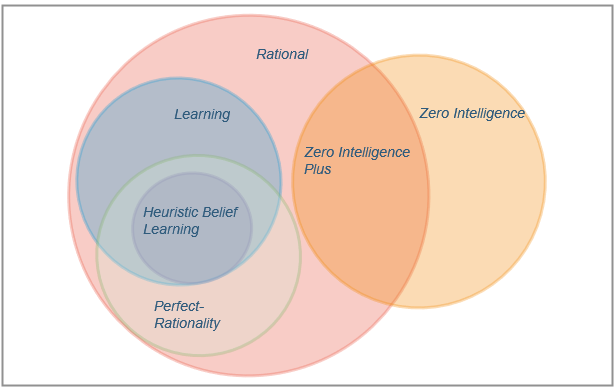
\includegraphics[scale=0.85]{agenci_venn.png}
\end{center}
\caption{Podstawowe klasy agentów na syntetycznych rynkach}\label{fig:agentsvenn}
\end{figure}
\end{center}
Finalnie modele agentowe często mają budowę będącą mieszanką koncepcji wywodzących się z rozwijanych wcześniej odrębnie wątków. Zbiór agentów w modelu ma charakter niejednorodny, zawiera różne typy agentów. Jest to uzasadnione istnieniem rzeczywistych grup graczy o odmiennych motywacjach (np. oczywistym podziałem jest podział na spekulantów i inwestorów długoterminowych). Dodatkowo zostało to również poparte analizą porównawczą, która wskazała, że modele ze zróżnicowanym zbiorem graczy znacząco lepiej odwzorowują stylizowane fakty nt. rynku niż modele oparte wyłącznie na agentach typu \textit{Zero Intelligence} \cite{getreal}. Spośród typów agentów występujących we współczesnych modelach agentowych możemy wyodrębnić kilka najbardziej istotnych klas (zobrazowanych również na rys. \ref{fig:agentsvenn}): 
\begin{itemize} 
\item agentów w pełni racjonalnych, których konstrukcja wywodzi się z teorii ekonomii lub jest bezpośrednim odwzorowaniem typowego działania wybranego uczestników rynku (\textit{Rational Agents}),
\item agentów składających zlecenia w sposób losowy, zdefiniowanych analogicznie do agentów modeli ekonofizycznych (\textit{Zero Intelligence Agent}),
\item agentów uczących się - zmieniających sposób działania na podstawie historii swoich dotychczasowych akcji (\textit{Learning Agents}), 
\item agentów aplikujących racjonalne reguły decyzyjne, ale częściowo zależnych od czynników losowych, np. wyznaczających cenę zlecenia zależnie od losowego czynnika(\textit{Zero Intelligence Plus Agents}).
\end{itemize} 
\subsection{Agenci typu \textit{Heuristic Belief Learning}}
Spośród agentów w pełni racjonalnych i uczących się szczególne znaczenie ma podklasa agentów typu HBL (\textit{Heuristic Belief Learning}) \cite{hblagent}. Agenci typu $HBL$ zostali wprowadzeni przez ekonomistów aspirujących do wyjaśnienia, w jaki sposób uczestnicy rynku z czasem uczą się wyznaczać cenę swoich ofert tak, aby możliwie szybko znaleźć kupca (sprzedawcę). Agent typu HBL wyznacza cenę planowanej oferty kupna i sprzedaży w oparciu o swoje oszacowanie szansy (przekonanie), że zlecenie wystawione po tej cenie jest najkorzystniejszym ruchem pod względem zysku i czasu realizacji. Formalizując, agent wyznacza cenę składanej oferty kupna lub sprzedaży na podstawie wzoru: 

$$p^*_i(t)= \left\{\begin{array}{lr}
        \mathrm{argmax}_p (p^i-p)f^i_t(p)& \text{dla kupna,}\\
        \mathrm{argmax}_p (p-p^i)f^i_t(p)& \text{dla sprzedaży,}\\
        \end{array}$$
gdzie:
\begin{itemize}
\item $p^i$ - indywidualna wycena $p^i$ handlowanego obiektu (instrumentu), może być zależna od czasu $t$ i liczby aktualnie posiadanych jednostek $\omega^i$, 
\item $f^i_t(p)$ - funkcja przekonania (ang.\textit{belief}) -  heurystyka prawdopodobieństwa, że zlecenie zostanie z sukcesem zrealizowane po cenie $p$, wyznaczana na podstawie historii dotychczasowych zleceń. 
\end{itemize}
Poważną wadą agentów typu HBL jest ich złożoność - ich konstrukcja wymaga stałego zapisywania i przechowywania wszystkich zleceń historycznych złożonych na giełdzie. Nawet jeśli ograniczymy okres zapisywanej historii, do np. $n$ ostatnich jednostek czasu, nadal jest to zadanie dosyć obciążające, szczególnie przy założeniu, że większość agentów (lub wszyscy, analogicznie do oryginalnego modelu \cite{hblagent}) niezależnie korzysta z tego mechanizmu wyznaczania ceny.
\subsection{Agenci typu \textit{Zero Intelligence Plus}}\label{sec:ziplus}
W tej pracy będziemy rozważać głównie agentów typu \textit{Zero Intelligence Plus} - agentów, których akcje mogą być, w różnym stopniu, losowe. Zakres pojęcia \textit{Zero Intelligence Plus} jest przy tym bardzo szeroki. Obejmuje minimalne modyfikacje agentów całkowicie losowych \textit{Zero Intelligence}, ale też agentów stosujących rozbudowane racjonalne strategie, z elementem losowości wprowadzonym jedynie na etapie wyznaczenia ceny, wielkości lub czasu wysłania zlecenia\cite{abides_explanation}.

W kontekście modeli rozważanych w tej pracy wyjątkowo ważne są dwa podtypy agentów \textit{Zero Intelligence Plus}\cite{lux}:
\begin{itemize}
\item agenci podejmujący decyzje w oparciu o obserwację danych rynkowych (ang. \textit{chartists} - "wykresiści"),
\item agenci podejmujący decyzję w oparciu o oszacowanie wartości instrumentu na podstawie wyceny indywidualnej oraz informacji "z zewnątrz" (ang. \textit{fundamentalists} - "fundamentaliści").
\end{itemize}
Powyższy podział jest odbiciem rzeczywistości - strategie graczy giełdowych możemy podzielić na bazujące głównie na wycenie instrumentu niezależnej od danych mikroekonomicznych (analiza fundamentalna) oraz na strategie polegające na wskaźnikach - funkcjach danych rynkowych mających identyfikować aktualne tendencje (analiza techniczna). 

Strategie "wykresistów" są, przy założeniu wiernego odwzorowania elementu instytucji $I$, możliwe do bezpośredniego przeniesienia na projekt agenta modelu. Decyzje podejmowane są na podstawie wskaźnika - funkcji danych rynkowych, które gracz może pozyskać za pomocą zapytania lub subskrypcji od agenta-giełdy $e^0$. Inaczej jest w przypadku drugiej grupy - "fundamentalistów", gdzie potrzebujemy do konstrukcji wprowadzić element subiektywnej wartości handlowanego obiektu dla agenta, z uwzględnieniem oszacowania na podstawie wiedzy publicznej oraz osobistych preferencji. W tym celu wprowadzamy do modelu dwa nowe obiekty: wartość fundamentalną instrumentu $r_t$ utożsamiającą wiedzę publiczną na temat wartości instrumentu oraz wektory wartości prywatnych agentów $\Theta = \{\theta^1, ..., \theta^m\}$ określające ich preferencje (przekonania o potencjalnym zaniżeniu lub zawyżeniu wartości). 
\subsubsection{Wartość fundamentalna}
Motywacją analizy fundamentalnej jest przekonanie, że cena rynkowa nie odzwierciedla dobrze rzeczywistej wartości instrumentu finansowego reprezentowanej przez $r_t$ - wartość fundamentalną. Zgodnie z założeniami, $r_t$ powinna utożsamiać całość aktualnej informacji publicznej na temat instrumentu, nie będąc przy tym podatną na spekulację powodującą fluktuacje ceny rynkowej. Teoretyczna wartość fundamentalna $r_t$ nie jest znana, stąd szacujemy jej wartość $\hat{r}_t$ korygując cenę rynkową w oparciu o zbiorczą informację z wielu źródeł.

Opisana powyżej logika przekłada się również na agentów realizujących strategie oparte na analizie fundamentalnej w ramach modelu: każdy z agentów tego typu ustala na swój użytek prywatną estymatę wartości fundamentalnej $\hat{r}^i_t$. Uściślenia wymaga jednak format informacji publicznej. Proces łączenia faktów z różnych źródeł jest pomijany: agenci za pośrednictwem dedykowanego obiektu - wyroczni $O$ obserwują wartość $r_t + \epsilon^i_t$, czyli wartość fundamentalną obarczoną błędem losowym i na jej podstawie aktualizują prywatne oszacowane $\hat{r}^i_t$.

W dotychczasowych modelach agentowych nie wyłoniła się spójna konwencja generowania danych udostępnianych agentom przez wyrocznię $O$. Część modeli używa w charakterze wyroczni danych historycznych, część definiuje $r_t$ jako proces stochastyczny. W tej pracy rozważamy jedynie drugie z podejść, przyjmując założenie że zawarta w modelu wyrocznia $O$ reprezentuje realizację parametryzowanego procesu stochastycznego. Szczegóły założonego procesu stochastycznego i estymacji $\hat{r}^i_t$ przez agentów opiszemy na przypadku modelu referencyjnego w kolejnym rozdziale.
% czy opisać orenstein -uhlenbeck już tutaj?
%Motywacją do wprowadzenia pojęcia wartości fundamentalnej do strategii inwestycyjnych jest przekonanie, że cena rynkowa nie odzwierciedla dobrze rzeczywistej wartości instrumentu finansowego - odbiega od sprawiedliwej ceny, stale zaniżając ją lub zawyżając. 
%znaleźć jakieś źródło z definicjami analizy technicznej i fundamentalnej 

% parę ogólnych zdań
% wkleić diagram Venna 
% przyjęcie notacji 
%ZI vs racjonalni, w tym HBL - przegląd 
\subsubsection{Preferencje}\label{sec:preferences}

Preferencje agentów wyrażamy przy pomocy atrybutu wartości prywatnych $\theta^i$. Wartości prywatne wywodzą się z teorii aukcji \cite{auction_theory}. 

Zgodnie z teorią aukcji wartość prywatna reprezentuje indywidualną dla agenta wycenę obiektu aukcji. Z wykorzystaniem pojęcia wartości prywatnych zostało wyprowadzonych kilka modeli przekonań i wiedzy licytujących graczy. W dziedzinie modeli agentowych wykorzystywany jest przede wszystkich podstawowy model - model niezależnych wartości prywatnych (ang. \textit{independent private values}, IPV). 
Model IPV definiuje wyceny obiektu poszczególnych graczy $(V_1,..., V_m)$ jako niezależne zmienne losowe o rozkładach odpowiednio $F_1, F_2, ..., F_m$. W konsekwencji niezależności zmiennych losowych, poszczególni gracze nie znają nawzajem swoich prywatnych wycen. 

Pierwotnie model niezależnych wartości prywatnych został sformułowany dla tradycyjnych jednostronnych aukcji pojedynczego obiektu. Przyjmujemy wówczas, że każdy gracz przystępuje do aukcji z prywatną wyceną $v_i$ wylosowaną odpowiednio z rozkładu $F_i$ i podejmuje decyzje o uczestnictwie w licytacji w oparciu o funkcję użyteczności $u^i$ następującej postaci:
$$u^i(p) = v_i - p, $$
gdzie $p$ jest aktualną ceną. 

Giełda reprezentuje bardziej złożony typ aukcji - aukcję ciągłą obustronną (ang. \textit{continous double auction}, CDA). Model modyfikujemy więc na potrzeby modelowania sesji giełdowej \cite{lobspoofing}, adresując przy tym dwa problemy: 
\begin{enumerate}
\item Możliwość kupna (sprzedaży) wielu jednostek instrumentu.
\item Możliwość zmiany wartości fundamentalnej instrumentu w trakcie trwania aukcji. 
\end{enumerate}
Pierwszy z problemów rozwiązujemy zastępując pojedynczą wartość wyceny $v_i$ wektorem wartości $v^i = (v^i_1, v^i_2, ...v^i_l)$ z rozkładu $F_i$, określającym wycenę każdej kolejnej dokupionej (sprzedanej) jednostki (przy założeniu możliwego kupna maksymalnie $l$ jednostek). Odpowiedzią na drugi problem jest rozbicie wyceny $v^i_j$ na dwa niezależne komponenty: 
$$v^i_j = r_t + \theta^i_j, $$
gdzie $r_t$ jest aktualną wartością fundamentalną handlowanego instrumentu, natomiast $\theta^i_j \in \theta^i$ wyraża preferencję zakupu $j$-tej jednostki. 
Scalając oba powyższe pomysły i dokładając możliwość handlu w dwie strony (kupna i sprzedaży równocześnie) wyposażamy $i$-tego gracza w następujący wektor preferencji $\theta^i$: 
$$\theta^i = (\theta^i_{-s}, \theta^i_{-j+1}, ...,\theta^i_{0}, ...,\theta^i_{l-1}, \theta^i_{l}),$$
gdzie $s$ - maksymalna liczba jednostek, które agent $i$ może sprzedać,$l$ - maksymalna liczba jednostek, które agent $i$ może kupić. Wartości $\theta^i_j\in \theta^i$ są z rozkładu $F'_i$. Zwykle przy stosowaniu w modelu agentowym przyjmujemy założenie $\theta^i_{j_1} \leq \theta^i_{j_2}$ dla $j_1 \leq j_2$, tzn. zakładamy że każda kolejna nabyta jednostka jest dla gracza mniej warta od poprzedniej. 

Dopuszczamy dużą elastyczność w interpretacji $v^i$ i $\theta^i$. Można użyć wartości prywatnych do zobrazowania nieracjonalnych sympatii, ale można też użyć jej do rozróżnienia różnego poziomu wiedzy specjalistycznej między graczami. W klasycznym sprawiedliwym modelu rynku, w którym zakładamy równy dostęp do informacji preferencje $\theta^i$ przyznajemy graczom w sposób losowy, z reguły przyjmując wspólny rozkład $\tilde{F}$ dla wszystkich graczy. Dla każdego gracza generujemy próbę losową rozmiaru wektora $\theta^i$, $|\theta^i| = s+k$, następnie sortujemy ją rosnąco, by zachować założenie o maleniu chęci kupna wraz ze zwiększaniem się liczby posiadanych jednostek.


\chapter{Model referencyjny}

Ze względu na złożoność procesu tworzenia modelu agentowego rynku od podstaw, zdecydowaliśmy się wesprzeć istniejącym modelem agentowym rynku opartego na arkuszu zleceń - ABIDES-em (\textit[Agent-Based Discrete Event Simulator}\cite{abides}). Użycie modelu referencyjnego ma na celu przede wszystkim ominięcie żmudnego procesu kalibracji (dopasowania konfiguracji do prawdziwych danych rynkowych w celu możliwie najlepszego odtworzenia rzeczywistości). Zakładamy, że konfiguracja referencyjna przedłożona przez autorów modelu referencyjnego dobrze odwzorowuje rzeczywistość i koncentrujemy się na rozszerzeniu istniejącego modelu pod kątem modelowania przewagi informacji, przypadku nieuwzględnionego w pierwotnej wersji. 

% sprawdzić dokładnie ABIDESA
Wybrany przez nas framework - ABIDES z założenia miał być narzędziem udostępnionym publicznie na zasadzie \textit{open-source} i służyć do rozwoju projektowania agentów. Od czasu publikacji został wielokrotnie wykorzystany w publikacjach autorów, m.in. do uczenia agentów przy pomocy metod reinforcement learning \cite{abides_reinforcement} czy weryfikowania hipotez na temat wpływu strategii arbitrażowych na zmienność ceny \cite{abides_arbitrage}.

W tej pracy decydujemy się na rozszerzenie modelu w kierunku testowania hipotez związanych z istnieniem przewagi informacyjnej wśród graczy. Zanim jednak przejdziemy do opisu wprowadzonego rozszerzenia i wyjściowych hipotez, nakreślimy działanie modelu referencyjnego. W pierwszej kolejności przyjrzymy się, jakie rozwiązania techniczne zostały zastosowane oraz w jaki sposób przytoczona wcześniej teoria dotycząca projektowania agentów znalazła odzwierciedlenie w implementacji. Następnie opiszemy zaproponowaną przez autorów konfigurację referencyjną, która posłuży nam za bazowy model rynku.

\section{Rozwiązania techniczne} 
\subsection{Chronologia zdarzeń}
W poprzednich rozdziałach skupiliśmy się głównie na elementach modelu specyficznych dla jego zastosowania do modelowania rynku, w domyśle przyjmując, że w symulacji przy pomocy modelu zagwarantowana jest poprawna chronologia zdarzeń. 

W kontekście chronologii zdarzeń warto podkreślić istnienie dwóch odrębnych grup symulatorów: działających w czasie rzeczywistym oraz nie działających w czasie rzeczywistym. Obie grupy cechują inne trudności w zachowaniu prawidłowej chronologii zdarzeń inicjowanych przez agentów. W kontekście modeli agentowych rynku najczęściej implementuje się je przy pomocy symulatorów nie działających w czasie rzeczywistym - w większości przypadków współczesnych zastosowań modeli agentowych motywacją jest sprawdzenie strategii inwestycyjnych lub hipotez na temat hipotetycznych zdarzeń, zatem dążymy do uzyskania możliwie największej próby symulacji. 

Wybrany model referencyjny ABIDES został zbudowany na bazie konceptu \textit{Discrete Event-Based Kernel}\cite{handbook_of_simulation}. W tej metodzie symulacja przebiega w dyskretnych krokach, a centrum symulacji stanowi jądro symulacji pośredniczące w każdym wydarzeniu zachodzącym w trakcie trwania symulacji. Jądro utrzymuje kolejkę priorytetową wszystkich wiadomości wysyłanych przez agentów (czyli, zgodnie z założeniami sekcji \ref{sec:language}, wszystkich wydarzeń zachodzących w symulacji) z kluczem czasu rosnąco. W każdym kroku ustala obowiązujący czas na podstawie najświeższej możliwej wiadomości $m$ i wywołuje metody odpowiedzialne za wykonanie akcji, którą $m$ utożsamia. 
\ref{fig:kerneluml}
\begin{center}
\begin{figure}
\begin{center}
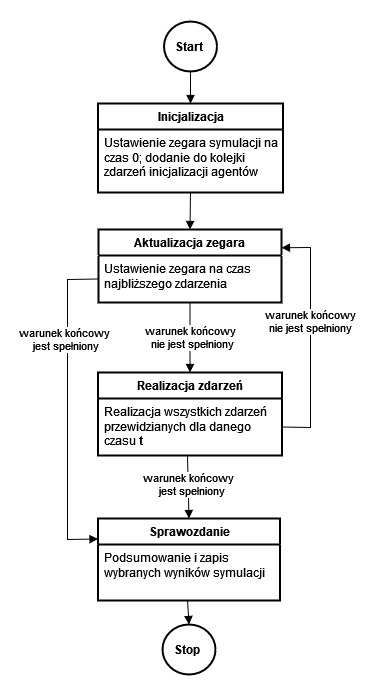
\includegraphics[scale=0.75]{kernel_uml.jpg}
\end{center}
\caption{Ogólny schemat przebiegu pojedynczej symulacji w metodzie \textit{Discrete Event-Based Kernel}, rysunek odwzorowany z \cite{handbook_of_simulation}}\label{fig:kerneluml}
\end{figure}
\end{center}

\subsection{Wyrocznia}

Autorzy ABIDES-a przyjmują założenie, że za zmianę wartości fundamentalnej odpowiada proces stochastyczny typu \textit{mean-reverting}. W dyskretnym wariancie jest on zdefiniowany przez poniższy wzór rekurencyjny \cite{wahwellman}: 
$$r_t = \max\{0,\kappa \bar{r} + (1+\kappa) r_{t-1} + u_t\}; r_0 = \bar{r}, $$
gdzie:
\begin{itemize}
\item $\bar{r}$ - średnia wartość fundamentalna,
\item $\kappa \n [0,1]$ - średni współczynnik powracania,
\item $u_t \sim N(0,\sigma_s)$ - błąd losowy.
\end{itemize}

Procesy typu \textit{mean reversion} dobrze odzwierciedlają cenę w krótkim zakresie czasu \cite{meanreversion} - zakładamy, że, póki nie dojdzie do istotnego w kontekście spółki wydarzenia ekonomicznego, cena stale oscyluje wokół średniej (uczciwej) wartości $\bar{r}$.

Opisany powyżej proces dyskretny ma poważną wadę w kontekście symulacji - jest relatywnie kosztowny obliczeniowo. Obliczenie $r_k$ wymaga obliczenia również $k-1$ poprzednich wartości. Jeśli weźmiemy pod uwagę, że domyślną jednostką symulacji w ABIDES-ie jest nanosekunda, często pojedyncza symulacja będzie wymagała obliczenia $8,64 \times 10^{13}$ kroków, bez względu na złożoność modelu agentowego - wystarczy by jeden z agentów zdecydował się skorzystać z informacji wyroczni w jednym z ostatnich kroków symulacji. Z tego względu w symulatorze zostaje wykorzystany proces stochastyczny ciągły proces Ornsteina-Uhlenbecka \cite{ouprocess}, który możemy traktować jako uogólnienie procesu typu \textit{mean reversion}. 
\subsection{Wielkość zleceń}
W modelu referencyjnym zakładamy istnienie pośród graczy kilku frakcji inwestorów, przy czym każdą frakcję cechuje inny rozkład wielkości zlecenia. Innymi słowy, przyjmujemy założenie, że rozmiar zlecenia składanego przez gracza $\omega$ jest zmienną losową o rozkładzie zdefiniowanym przez mieszankę rozkładów: w pierwszej kolejności przydzielamy graczowi grupę według zamożności zgodnie z prawdopodobieństwami przynależności do jednej z $m$  frakcji $\pi=\{\pi_1,...,\pi_f\},\sum_{i \in [f]} \pi_i =1$, w drugiej kolejności losujemy rozmiar złożonego zlecenia z rozkładu właściwego grupie $f_i$ (tabela \ref{tab:distmix}).

\begin{table}
\caption{Frakcje graczy i ich rozkłady zleceń} 
\label{tab:distmix}
% opisać modify, replace, partial cancel, złożenie 
\begin{center}
\begin{tabular}{ |p{2cm}|p{10cm}|}
\hline
\textbf{$\pi_i$} & \textbf{$f_i$} \\
\hline 0,2 & rozkład logarytmicznie normalny $\mathrm{Lognormal}(\mu=2.9, \sigma^2=1.2)$\\
\hline
 0,7 & rozkład normalny $N(\mu=100, \sigma^2=0.15)$\\
 \hline
 0,06& rozkład normalny $N(\mu=200, \sigma^2=0.15)$\\
 \hline
0,004& rozkład normalny $N(\mu=300, \sigma^2=0.15)$\\
\hline
0,0329 & rozkład normalny $N(\mu=400, \sigma^2=0.15)$\\
\hline
0,001 & rozkład normalny $N(\mu=500, \sigma^2=0.15)$\\
\hline
0,0006 &rozkład normalny $N(\mu=600, \sigma^2=0.15)$\\
\hline
0,0004 &rozkład normalny $N(\mu=700, \sigma^2=0.15)$\\
\hline
0,0005 &rozkład normalny $N(\mu=800, \sigma^2=0.15)$\\
\hline
0,0003 &rozkład normalny $N(\mu=900, \sigma^2=0.15)$\\
\hline
0,0003 & rozkład normalny $N(\mu=1000, \sigma^2=0.15)$\\
\hline
\end{tabular} 
\end{center}
\end{table}
% dać tabelę [prob frakcji][rozkład]
% ewentualnie dopisać tu jakiesś zdanie
\subsection{Implementacja}
Implementacja nie odwzorowuje bezpośrednio teoretycznego podziału na $I$ - instytucję i $E$ - środowisko wprowadzonego w rozdziale 2. (sekcja \ref{sec:theoreticalmodel}), obiekty współtworzące model w swoich atrybutach i metodach mieszają elementy obu teoretycznych warstw. 

Model referencyjny ABIDES został napisany obiektowo. Typy agentów są zdefiniowane w postaci klas. Hierarchię klas agentów w modelu obrazuje schemat \ref{fig:classdiagram}. 
\begin{center}
\begin{figure}
\begin{center}
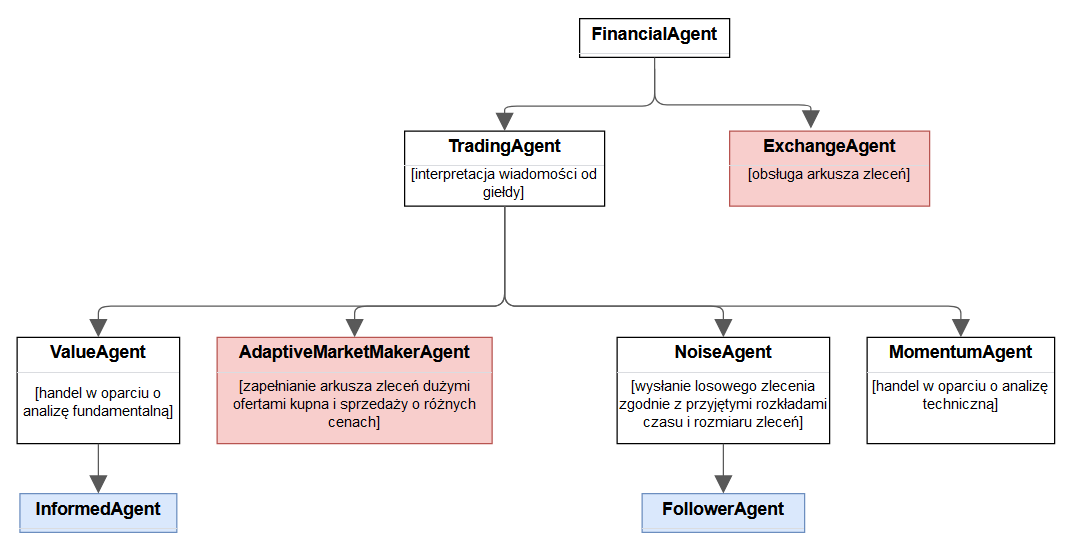
\includegraphics[scale=0.7]{schemat_klas_2.png}
\end{center}
\caption{Schemat klas w modelu i ich podstawowe funkcjonalności. Kolorem czerwonym oznaczeni zostali agenci specjalni (nie modyfikujący strategii), kolorem niebieskim oznaczeni zostali nowo wprowadzeni agenci.}\label{fig:classdiagram}
\end{figure}
\end{center}
Nie będziemy omawiać większości metod i atrybutów klas. Skoncentrujemy się na dwóch kluczowych metodach, które zawierają w sobie całość strategii wybranego typu agenta:
\begin{itemize}
\item \textit{onWakeup} - odpowiada funkcji determinującej aktywność $i.$ gracza $g^i(t_0,t,T)$; określa działania podejmowane przez agenta w momencie obudzenia,
\item \textit{onReceive} - łączy w sobie funkcje alokacji $h^i(m)$ i kosztu $c^i(m)$; określa reakcje agenta na otrzymywane wiadomości, w szczególności aktualizuje stan środków agenta po otrzymaniu potwierdzenia realizacji zlecenia.
\end{itemize}


\section{Konfiguracja referencyjna}

W kontekście celów postawionych w tej pracy najbardziej użytecznym elementem modelu referencyjnego jest załączona do niego konfiguracja referencyjna RMSC04. Kalibracja modelu agentowego, czyli dostosowanie jego parametryzacji w taki sposób, by możliwie najwierniej odzwierciedlał rzeczywistą sytuację, jest, sama w sobie, trudnym i czasochłonnym procesem. Spośród problemów z jakimi należy się zmierzyć w trakcie kalibracji modelu możemy wymienić sposób mierzenia podobieństwa między rzeczywistą sytuacją a próbą jej odwzorowania w symulacji oraz dobór zbioru konfiguracji spośród których będziemy wybierać optymalną. Z wymienionych przyczyn, trudno byłoby włączyć etap kalibracji modelu w zakres pracy. 

Konfiguracja referencyjna RMSC04 (tabela \ref{tab:refconfig}) jest konfiguracją opracowaną przez jego autorów w momencie rozszerzenia frameworku o tworzenie w oparciu o model agentowy środowisk do uczenia agentów uczonych przez wzmacnianie (reinforcement learning) \cite{abides_gym}. Wzorowana jest na rynkach giełdy amerykańskiej giełdy papierów wartościowych NASDAQ\cite{nasdaq} i zawiera wyłącznie agentów typu Zero Intelligence oraz Zero Intelligence Plus. 

Niestety, w swoich pracach oraz w repozytorium symulatora, autorzy ABIDES-a nie opisali procesu kalibracji modelu czy też uzasadnienia zmian, jakich dokonali względem pierwotnej konfiguracji RMSC03, załączonej do pierwszej wersji symulatora \cite{getreal}. W RMSC04 wprowadzono jedną znaczącą zmianę względem RMSC03 - wykluczono z niej agentów typu Heuristic Belief Learning, przypuszczalnie głównie z powodów wydajnościowych (przyp. agenci typu HBL wymagają pobierania danych o wszystkich zleceniach z ustalonego okresu $T$ w każdym kroku). 

\begin{table}
\caption{Skład konfiguracji referencyjnej RMSC04}\label{tab:refconfig}
\begin{center}
\begin{tabular}{|p{3cm}|p{3cm}|p{4cm}|p{3cm}|}
\hline
\textbf{klasa agenta} & \textbf{typ agenta} & \textbf{model obudzeń} & \textbf{liczba agentów}\\
\hline
ExchangeAgent & - & - & 1\\
\hline
AdaptiveMarketMakerAgent & Zero Intelligence Plus & narzucona częstotliwość: 60s &1\\
\hline
ValueAgent & Zero Intelligence Plus & proces Poissona z $\lambda=5.7^{-12}$ & 102\\
\hline
MomentumAgent & Zero Intelligence Plus & narzucona częstotliwość: 60s & 12 \\
\hline
NoiseAgent & Zero Intelligence & zgodnie z rozkładem U-kwadratowym&1000\\
\hline
\end{tabular} 
\end{center}
\end{table}

Wybrana konfiguracja referencyjna zawiera agentów pięciu różnych typów (klas), z czego dwóch specjalnych (oznaczonych również na schemacie \ref{fig:classdiagram}): \textit{ExchangeAgent} oraz \textit{AdaptiveMarketMakerAgent}. ExchangeAgent to agent - giełda, którego jedynym zadaniem jest obsługa rynku (arkusza zleceń) i nie uczestniczy w transakcjach kupna lub sprzedaży jako strona. Z kolei AdaptiveMarketMakerAgent to agent reprezentujący animatora rynku (ang. \textit{market makera}), czyli współpracujący z giełdą podmiot mający zapewnić ciągłość handlu na giełdzie poprzez zobowiązanie do składania regularnie równocześnie ofert kupna i sprzedaży spełniających umówione kryteria pod względem m.in. cen i wielkości ofert. Animator rynku, poza zyskiem z handlu instrumentem, może również otrzymywać wynagrodzenie ze strony giełdy lub emitenta papierów wartościowych, czego model agentowy rynku nie uwzględnia. Obaj gracze realizują ustalone akcje, których nadrzędnym celem jest płynne działanie rynku, ich sposób działania nie podlega modyfikacji. Używając terminu \textit{gracze} o agentach modelu, będziemy domyślnie pomijać agentów wspomnianych klas.

Pozostałe trzy klasy agentów uwzględnione w konfiguracji referencyjnej to typy agentów podobne do występujących już wcześniej w literaturze. \textit{NoiseAgent} to minimalnie zmodyfikowany klasyczny agent Zero Intelligence, wysyłający losowe zlecenia. Natomiast klasy \textit{ValueAgent} i \textit{MomentumAgent} nawiązują do podziału na agentów podejmujących decyzje w oparciu o analizę techniczną oraz agentów podejmujących decyzję w oparciu o analizę fundamentalną, opisanego szerzej w sekcji \ref{sec:ziplus}

\chapter{Modelowanie przewagi informacji}
Większość modeli agentowych jest zbudowanych w zgodzie z dwoma założeniami, wynikającymi w dużej mierze z zaadaptowania metod zaczerpniętych z teorii aukcji (model IPV): 
\begin{enumerate}[I.]
\item \textbf{Równy dostęp do informacji}
\item \textbf{Niezależność i prywatność preferencji}
\end{enumerate}
W konsekwencji powyższych założeń, klasyczne modele agentowe rynku wykluczają wymianę informacji między agentami na temat stanu wiedzy i preferencji, znacząco przy tym upraszczając model i zawężając zbiór strategii graczy. Wyłączone również są przypadki, gdy wśród inwestorów dostęp do informacji jest zróżnicowany. 

Przenosząc powyższe założenia bezpośrednio na współczesne realia, możemy zauważyć, że istnieją przesłanki by je zakwestionować. W przeszłości głównym źródłem nierówności w wiedzy na temat wartości spółki był proceder tzw. \textit{insider tradingu} - wykorzystywania w handlu uprzywilejowanego dostępu do niepublicznej informacji. Współcześnie, w dobie zaawansowanych modeli predykcyjnych ceny, sytuacja nie jest tak jednoznaczna - przewaga informacji może wynikać z przewagi technologicznej. Również założenie niezależności i prywatności preferencji budzi oczywiste wątpliwości w kontekście odnotowywanych reakcji na publikowane w mediach społecznościowych rekomendacje czy też, coraz bardziej zauważalnych, prywatnych grup lub forów publikujących rekomendacje inwestycyjne. Z takimi motywacjami podejmujemy próbę uzupełnienia standardowego modelu o mechaniki zróżnicowania wiedzy między graczami oraz komunikacji między nimi. 

\section{Założenia}\label{sec:assums}
% powprowadzać parametry

Nie sposób ująć w jednym modelu wszystkie występujące zjawiska wynikające z nierównego dostępu do informacji i dzielenia się przekonaniami, zaczynamy więc od narzucenia ograniczeń na planowane rozszerzenie modelu.  

\subsection{Zdarzenie}
Zgodnie ze stylizowanymi faktami na temat rynku (Fakt \ref{fact:events}) zakładamy, że cena $p$ obowiązująca na rynku jest podatna na tzw. zdarzenia ekonomiczne, wiążące się z upublicznieniem danych wpływających na wartość instrumentu. 

Na potrzeby wprowadzenia prostego modelu przewagi informacji, założymy że w założonym zakresie czasowym symulacji $[t_0, T]$ dochodzi do zdarzenia $\eta = (t_{\eta},\Delta_{r})$, gdzie $t_{\eta}$ - czas zdarzenia, $\Delta_{r}$ - wynikająca z niego zmiana wartości fundamentalnej $r_t$ instrumentu. Dodatkowo przyjmujemy, że czas zdarzenia (publikacji) $t_{\eta}$ jest ustalony z wyprzedzeniem. 

Technicznie, powyższe założenia realizujemy modyfikując ciąg wartości fundamentalnych $r_t$ generowanych przez wyrocznię $O$ - zwiększając wartość $r_{t_{\eta}}$ o wartość $\Delta_{r}$ (w konsekwencji również kolejne $r_t$ dla $t>t_{\eta}$). Zdarzenie $\eta$ wprowadzamy jako parametr modelu. 

% rozważyć wrzucenie wykresu
\subsection{Informatorzy i obserwujący}
Zbiór klas agentów modelu rozszerzamy o dwa nowe typy agentów:
\begin{itemize}
\item \textit{InformedAgent} - informatorów, dysponujących wiedzą na temat nadchodzącego zdarzenia,
\item \textit{FollowerAgent} - obserwujących, postępujących zgodnie z rekomendacją daną przez obserwowanego informatora. 
\end{itemize}
Oba typy agentów częściowo bazują na klasach już istniejących w modelu (zgodnie ze  schematem \ref{fig:classdiagram}). 

Informator \textit{InformedAgent} bazuje na klasie \textit{ValueAgent} - agenta uzależniającego swoją strategię od obserwowanej wartości fundamentalnej. Informator dziedziczy po nim model obudzeń oparty na procesie Poissona oraz sposób estymacji finalnej wartości fundamentalnej ($r_T$ - wartości fundamentalnej na koniec założonego okresu czasu; sposób estymacji opisany szerzej w \cite{abides_explanation}). 

Z kolei obserwujący \textit{FollowerAgent} jest rozwinięciem agenta Zero Intelligence \textit{NoiseAgent}. Dziedziczy po nim model obudzeń oparty na rozkładzie U-kwadratowym oraz losowy rozmiar zlecenia zgodny z mieszanką rozkładów (daną tabelą \ref{tab:distmix}).

Wprowadzenie do modelu graczy informatorów i graczy obserwujących ma umożliwić modelowanie sytuacji, w której wokół osoby uprzywilejowanej dodatkową wiedzą skupia się grono obserwujących (np. subskrybentów płatnej grupy lub forum). Stąd, zakładamy, że obserwujący nie są zainteresowani preferencjami innych obserwujących. W konsekwencji graf komunikacji między obserwującymi a informatorem ma topologię gwiazdy. 
% rozważyć wrzucenie grafu-gwiazdy [lub grafu złożonego z kilku gwiazd]

\section{Uwzględnienie przewagi informacji}
Do celów uwzględnienia przewagi informacji wykorzystamy obiekt wartości prywatnych $\theta^i$ gracza (sekcja \ref{sec:preferences}), równocześnie wprowadzając ten element do modelu referencyjnego. Wartości $\theta^i$ wyznaczymy korzystając z założeń przyjętych w sekcji \ref{sec:assums}, a konkretnie ustalenia zdarzenia $\eta = (t_{\eta}, \Delta_r)$ jako parametru symulacji. W oparciu o dane zdarzenie $\eta$, wartości $\theta^i$ wyznaczamy jako próbkę z rozkładu o wartości oczekiwanej $\mu_{theta} = \Delta_r$ oraz wariancji $\sigma^2_{\theta}$ zależnej od wprowadzonego parametru niepewności oszacowania informatora. 

Uogólniając, różnicujemy przewagę informacji poprzez zróżnicowanie rozkładów wartości prywatnych agentów $F'_i$ (przede wszystkim ich wartości oczekiwanych).

\section{Komunikacja między agentami}

Komunikacja między obserwującymi agentami a informatorem odbywa się z wykorzystaniem mechanizmu zapytania. Agent obserwujący wysyła do informatora prośbę o udzielenie rekomendacji \textit{QuerySideRecommendation}. W odpowiedzi agent informator dodaje prośbę do kolejki oczekujących, rekomendację wyznaczając i wysyłając po pobraniu aktualnych cen przy kolejnym obudzeniu (Algorytm \ref{alg:informer}). 
\begin{pseudokod}
\caption{\textit{InformedAgent: onReceive}}\label{alg:informer}

\KwData{$m \in M$, $s_m \in [n],t_m \in [t_0, T], \xi \in \Xi$}
\vspace{0.5cm}
\If{$m = \text{\textit{QuerySideRecommendation}}$}{
pendingRequests.put(($t_m$, $s_m$))\tcp*[r]{kolejka oczekujących próśb}
}
\vspace{0.5cm}
\If{$\xi = \text{\textit{AWAITING\_SPREAD}}$}{
\If{$m = \text{\textit{QuerySpreadResponseMsg}}$}{
placeOrder()\tcp*[r]{agent realizuje swoje cele}
sendPendingRecommendations()\tcp*[r]{agent realizuje rekomendacje}
$\xi := \text{\textit{AWAITING\_WAKEUP}}$\;
}
}
\end{pseudokod}

\begin{pseudokod}
\caption{\textit{FollowerAgent: onReceive}}\label{alg:follower}

\KwData{$m \in M$, $s_m \in [n],t_m \in [t_0, T], \xi \in \Xi$}
\vspace{0.5cm}
\If{$\xi = \text{\textit{AWAITING\_SIGNAL}}$}{
\If{$m = \text{\textit{TradingSignal}}$}{
\eIf{$m=\text{\textit{BID}}$}{
$o_s := \textit{BID}$\tcp*[r]{interpretacja rekomendacji}
}{\If{$m=\text{\textit{ASK}}$}{
$o_s := \textit{ASK}$;\
}
}
sendMessage(\textit{QuerySpreadMsg});\\
$\xi := \text{\textit{AWAITING\_SPREAD}}$;\

}}
\vspace{0.5cm}
\If{$\xi = \text{\textit{AWAITING\_SPREAD}}$}{
\If{$m = \text{\textit{QuerySpreadResponseMsg}}$}{
placeOrder(side=$o_s$)\tcp*[r]{wykorzystanie rekomendacji}
$\xi := \text{\textit{AWAITING\_WAKEUP}}$;\\
}}

\end{pseudokod}
Rekomendacje informatora mają charakter dyskretny: zwracana jest wiadomość \textit{ASK}("SPRZEDAJ") lub \textit{BID} ("KUP") zgodnie z funkcją: 
$$
 R_t = 
 \left\{\begin{array}{lr}
        ASK, & \text{dla }p_t - \epsilon^I > \hat{r_t} +\theta^I_{\omega^I}\\
        BID, & \text{dla } p_t + \epsilon^I < \hat{r_t} +\theta^I_{\omega^I}\\
        NULL, & \text{w pozostałych przypadkach,}
        \end{array}

$$ 

gdzie:
\begin{itemize}
\item $R_t$ - rekomendacja w chwili $t$, 
\item $\hat{r_t} +\theta^I_{\omega^I}$ - aktualna wycena informatora, 
\item $\epsilon^I$ - margines niepewności przyjęty przez informatora.
\end{itemize}
Po otrzymaniu rekomendacji obserwujący agent wyznacza na jej podstawie stronę kolejnego zlecenia, a następnie wysyła zapytanie do agenta-giełdy o ceny kupna $a(t)$ i sprzedaży $b(t)$.

\chapter{Analiza wpływu przewagi informacji}
Posiadanie informacji niedostępnej dla pozostałych uczestników rynku bez wątpienia stawia informatora na wygranej pozycji - podczas gdy inni gracze muszą liczyć się z ryzykiem, zysk informatora jest praktycznie pewny. Pozornie oczywista strategia informatora komplikuje się jednak w ujęciu długoterminowym, trzeba wówczas rozważyć problemy pomijalne w kontekście jednorazowego incydentu wykorzystania przewagi informacyjnej. Przede wszystkim, trzeba wziąć pod uwagę, że inni gracze, będąc stratni, mogą zrezygnować z inwestowania na danym rynku lub zmodyfikować swoje strategie w sposób niekorzystny dla informatora. W obu przypadkach informator może długoterminowo stracić stosując najbardziej zyskowną strategię przy założonych stałych strategiach pozostałych graczy. 

Gruntowna weryfikacja optymalnej strategii informatora w zależności od kapitału i liczby obserwujących jest zadaniem kompleksowym - wymaga zdefiniowania alternatywnych do referencyjnej konfiguracji modelu. Rozważamy zatem analizę znacznie prostszą, ale pozwalającą nakreślić wpływ obecności informatora na rynek w zależności od skali jego działania i wskazać potencjalne ograniczenia jego strategii.

\section{Plan symulacji}

Eksperyment rozbijemy na dwa etapy. W pierwszej kolejności nie uwzględnimy obecności obserwujących agentów, skupiając się jedynie na wpływie obecności insidera i jego optymalnych strategiach w zależności od kapitału, jakim dysponuje. Następnie, dla ustalonego kapitału informatora włączymy do symulacji obserwujących agentów i przyjrzymy się, czy dzielenie się informacją jest dla niego korzystne. W obu etapach, dla uproszczenia, przyjmujemy taki sam model obudzeń informatora (generowanych, analogicznie jak w przypadku agentów klasy \textit{ValueAgent}, zgodnie z procesem Poissona zdefiniowanym w tabeli \ref{tab:refconfig}) oraz taki sam scenariusz wyroczni, tzn. przyjmujemy, że w każdym z testowanych przypadków zachodzi zdarzenie $\eta = (t_{\eta}, \Delta_r).$

\subsection{Zależność strategii od kapitału}
Celem strategii informatora jest kupno możliwie najtaniej (sprzedaż możliwie najdrożej) jednostek instrumentu przed oczekiwaną zmianą ceny. Podstawowymi cechami różnicującymi potencjalne strategie informatora są liczba i rozmiar zleceń, w jakich gracz realizuje swoje cele. Spośród zbioru strategii możemy wyróżnić dwie skrajne: dyskretnego informatora, który wykonuje w odstępach czasu szereg zleceń małej lub przeciętnej wielkości, oraz dominatora o praktycznie nieograniczonych środkach, wystawiającego bardzo duże, zauważalne, zlecenia.

Dwie skrajne strategie narzucają zakres planowanych symulacji. Możliwości finansowe informatora definiujemy parametrem \texttt{max\_qty} - maksymalną liczbą jednostek, które może nabyć (sprzedać), zakres ich możliwych wartości wyznaczamy na podstawie rozkładu zleceń. Możliwe rozmiary zleceń informatora \texttt{order\_size} wyznaczamy w oparciu o załączony do konfiguracji referencyjnej rozkład dany tabelą \ref{tab:distmix} - na tej podstawie szacujemy przeciętną oraz przypadki skrajne. 

Dla każdej z rozważanych wartości maksymalnej liczby jednostek \texttt{max\_qty} dobieramy trzy różne wartości \texttt{order\_size} mające odwzorowywać trzy różne realizacje kupna (sprzedaży) \texttt{max\_qty}: w możliwie najmniejszych zleceniach, w kilku partiach oraz w jednym dużym zleceniu. Dokładne wartości parametrów \texttt{max\_qty} i \texttt{order\_size} zostały zawarte w tabeli \ref{tab:simplan1}.
\begin{table}
\caption{Plan symulacji dla konfiguracji zależnych od rozmiaru zlecenia i maksymalnej liczby jednostek } 
\label{tab:simplan1}
% opisać modify, replace, partial cancel, złożenie 
\begin{center}
\begin{tabular}{|p{2cm}|p{2cm}|p{2cm}|}
\hline
\textbf{\texttt{max\_qty}} & \textbf{\texttt{order\_size}} & \textbf{liczba replikacji} \\
\hline 
100 & 5 & 25 \\
 & 25 & 25 \\
 & 100 & 25 \\
\hline
1000 & 25 & 25 \\
 & 250 & 25 \\
 & 1000 & 25 \\
\hline
10000 & 250 & 25 \\
 & 2500 & 25 \\
 & 10000 & 25 \\
\hline
10000000 & 25000 & 25 \\
 & 2500000 & 25 \\
 & 10000000 & 25 \\
\hline
\end{tabular} 
\end{center}
\end{table}
\subsection{Wpływ liczby obserwujących na strategię informatora}
Wartości parametrów \texttt{order\_size} i \texttt{num\_followers} - liczby obserwujących zostały zawarte w tabeli \ref{tab:simplan2}.
\begin{table}
\caption{Plan symulacji dla konfiguracji zależnych od rozmiaru zlecenia i liczby agentów obserwujących informatora} 
\label{tab:simplan2}
% opisać modify, replace, partial cancel, złożenie 
\begin{center}
\begin{tabular}{|p{2cm}|p{2cm}|p{2cm}|p{2cm}|}
\hline
\textbf{\texttt{max\_qty}} & \textbf{\texttt{order\_size}} & \textbf{liczba obserwujących} & \textbf{liczba replikacji} \\
\hline 
10000 & 25 & 10 & 25 \\
& & 50& 25\\
& & 100 & 25\\
& & 500& 25\\
& &1000 & 25\\
\hline
10000 & 100 & 10 & 25 \\
& & 50& 25\\
& & 100 & 25\\
& & 500& 25\\
& &1000 & 25\\
\hline
10000 & 1000 & 10 & 25 \\
& & 50& 25\\
& & 100 & 25\\
& & 500& 25\\
& &1000 & 25\\
\hline

\end{tabular} 
\end{center}
\end{table}



% tabele [liczba replikacji] [kolejne parametry]
%[tutaj opisuję, jakie konfiguracje testowałam w ilu próbach i dlaczego takie]
\section{Analiza wyników}
W pracy omówimy tylko najistotniejsze wnioski wynikłe z analizy wyników symulacji. Całość wyników oraz notatniki podsumowujące całość zebranych danych są załączone jako uzupełnienie pracy oraz udostępnione w \href{https://github.com/AgataCieslik/abides-jpmc-public}{publicznym repozytorium pracy} .
\subsection{Wpływ skali działania informatora na innowację ceny}
Zgodnie z oczekiwaniami, wyniki symulacji wykazują wpływ obecności informatora na kształtowanie się ceny. Przede wszystkim decydujące znaczenie ma tutaj wielkość zaangażowanych środków informatora (wyrażona parametrem \texttt{max\_qty}). Realizacja dużych transakcji znacząco przyspiesza proces uwzględnienia efektu zdarzenia w cenie (Rysunek \ref{fig:meanpriceinn}).
\begin{center}
\begin{figure}
\begin{center}
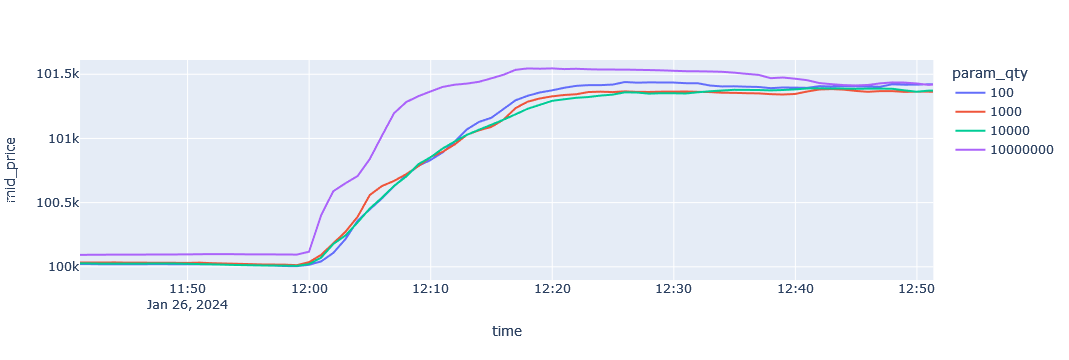
\includegraphics[scale=0.4]{srednia_innowacja_ceny.png}
\end{center}
\caption{Wykres średnich cen w replikacjach pogrupowanych według możliwości finansowania informatora}\label{fig:meanpriceinn}
\end{figure}
\end{center}
Również rozmiar i częstotliwość zleceń wydają się nie pozostawać bez wpływu na proces kształtowania ceny. Sytuację dobrze obrazuje wykres ceny w zależności od parametryzacji dla replikacji (równoważnej realizacji procesu wyroczni) o id 16 (Rysunek \ref{fig:priceinn}).
\begin{center}
\begin{figure}
\begin{center}
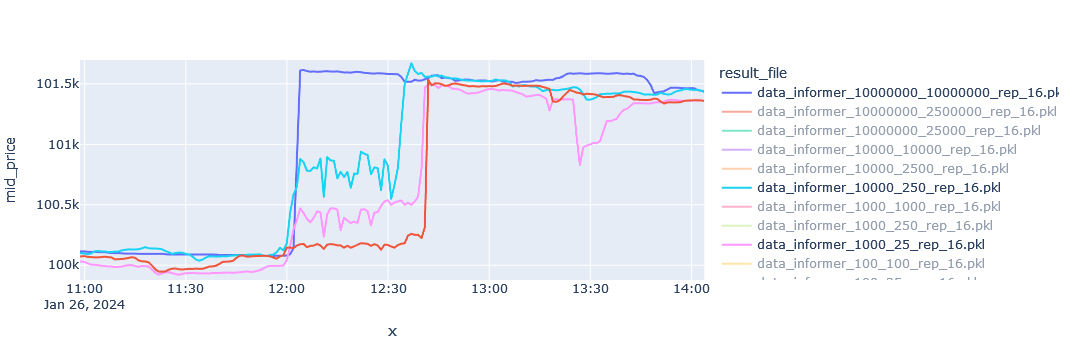
\includegraphics[scale=0.4]{innowacja_ceny.png}
\end{center}
\caption{Wykres ceny w zależności od parametryzacji informatora dla replikacji o id=16}\label{fig:priceinn}
\end{figure}
\end{center}
\subsection{Ograniczenie na maksymalny kapitał informatora} 
Porównując wyniki symulacji w zależności od zaangażowanego kapitału informatora możemy wysnuć hipotezę, że istnieje ograniczenie na maksymalny zaangażowany kapitał gracza z uprzywilejowaną informacją. 
\begin{center}
\begin{figure}
\begin{center}
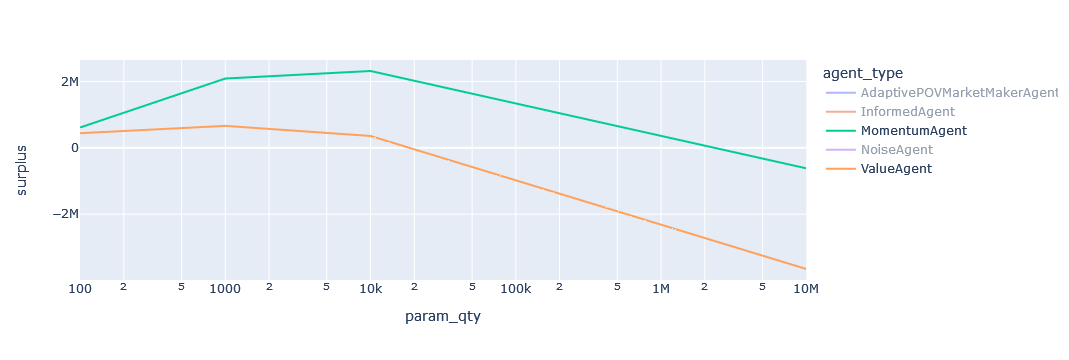
\includegraphics[scale=0.4]{kapital.png}
\end{center}
\caption{Średnie wypłaty agentów klas \textit{ValueAgent} i \textit{MomentumAgent} w zależności od zaangażowanych środków informatora}\label{fig:capital}
\end{figure}
\end{center}
Wnioski opieramy w głównej mierze na analizie wypłat dla graczy konfiguracji referencyjnej \textit{ValueAgent} i \textit{MomentumAgent} (Rysunek \ref{fig:capital}) reprezentujących dwa rzeczywiste nurty inwestowania: strategie oparte na analizie fundamentalnej oraz bazujące na analizie technicznej. Oba typy agentów odnotowują średnio znaczne straty dla maksymalnej wartości środków informatora, co budzi wątpliwości, czy w rzeczywistości zdecydowaliby się realizować do końca swój scenariusz inwestycyjny, równocześnie umożliwiając informatorowi dopełnienie jego strategii zgodnie z planem. 

\subsection{Wpływ strategii informatora na wypłaty innych graczy}
Analiza wyników symulacji wskazała ciekawy konflikt interesów między agentami typów \textit{ValueAgent} oraz \textit{MomentumAgent} - graczom tych typów sprzyjają dwie skrajne strategie informatora (dobrze to widać na przykładzie tabeli wypłat na rys. \ref{fig:gametab}). W przypadku \textit{ValueAgent} najkorzystniejszą strategią informatora jest strategia oparta na zleceniach relatywnie małych rozmiarów, w niewielkim stopniu wpływających na cenę. Z kolei dla agentów typu \textit{MomentumAgent} najkorzystniejsze są strategie wystawiające zlecenia dużych rozmiarów, które wpływają zauważalnie na cenę rynkową i skutkują zaktualizowaniem używanych przez agenta wskaźników analizy technicznej zgodnie z rzeczywistym kierunkiem zmiany ceny w przyszłości. 
\begin{center}
\begin{figure}
\begin{center}
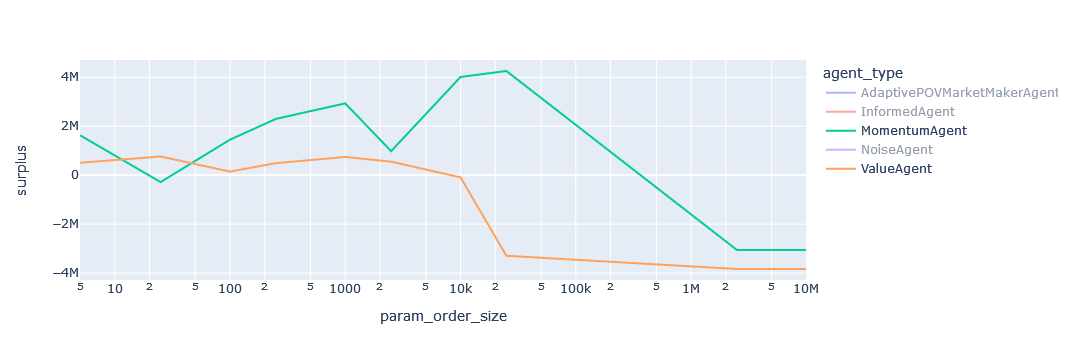
\includegraphics[scale=0.4]{ordersize.png}
\end{center}
\caption{Średnie wypłaty agentów klas \textit{ValueAgent} i \textit{MomentumAgent} w zależności od wielkości zleceń informatora}\label{fig:ordersnum}
\end{figure}
\end{center}
\begin{center}
\begin{figure}
\begin{center}
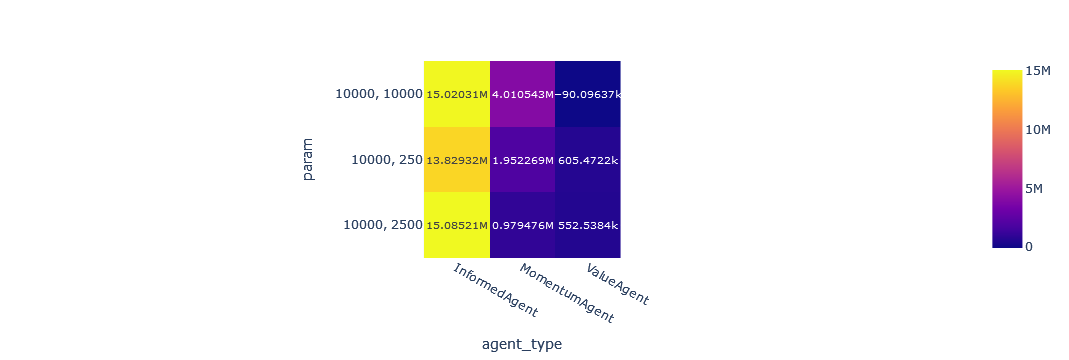
\includegraphics[scale=0.4]{table.png}
\end{center}
\caption{Tabela wypłat graczy dla ustalonego parametru informatora \texttt{max\_qty}=10000}\label{fig:gametab}
\end{figure}
\end{center}
\subsection{Ograniczenie na liczbę obserwujących}
Analiza konfiguracji z włączonymi populacjami agentów - obserwatorów informatora sugeruje, że informator powinien narzucić ograniczenie na rozmiar grupy, której udostępnia rekomendacje. Sporządzone wykresy średnich wypłat (rys.\ref{fig:followers}) zarówno informatora, jak też jego obserwatorów, jasno pokazują, że powyżej 50 agentów w populacji obserwatorów średnie wypłaty obu typów agentów maleją.
\begin{center}
\begin{figure}
\begin{center}
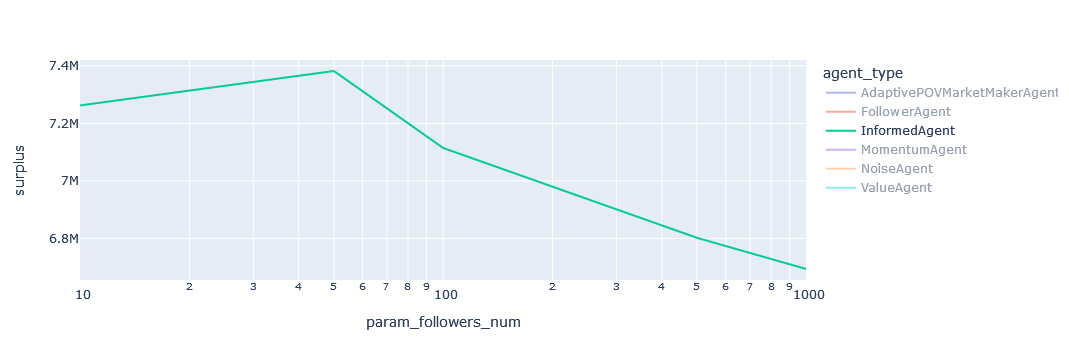
\includegraphics[scale=0.4]{informer_by_fnum.png}
\end{center}
\begin{center}
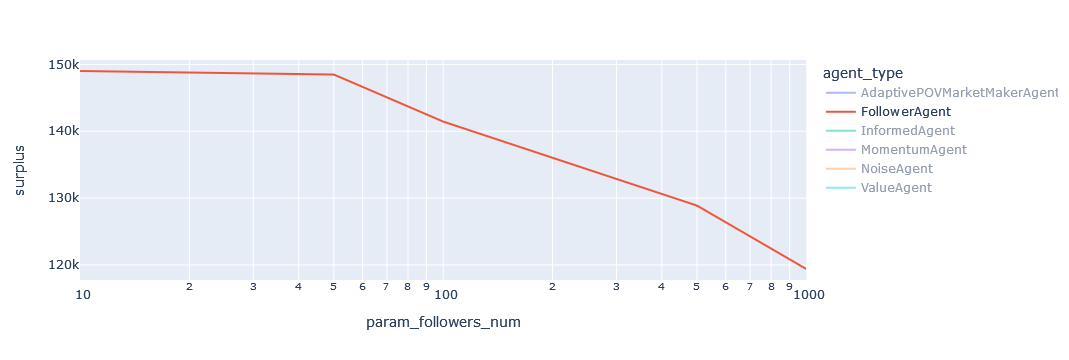
\includegraphics[scale=0.4]{follower_by_fnum.png}
\end{center}
\caption{Średnie wypłaty informatorów i obserwatorów w zależności od liczby obserwujących informatora}\label{fig:followers} 
\end{figure}
\end{center}
Prawdopodobnym uzasadnieniem tej zależności jest występowanie dla dużych grup obserwatorów małych baniek spekulacyjnych (rys. \ref{fig:ball}) - duża grupa obserwatorów równocześnie realizujących swoje zlecenia zgodnie z przyjętą bezkrytycznie rekomendacją winduje cenę ponad rzeczywistą wartość instrumentu.
\begin{center}
\begin{figure}
\begin{center}
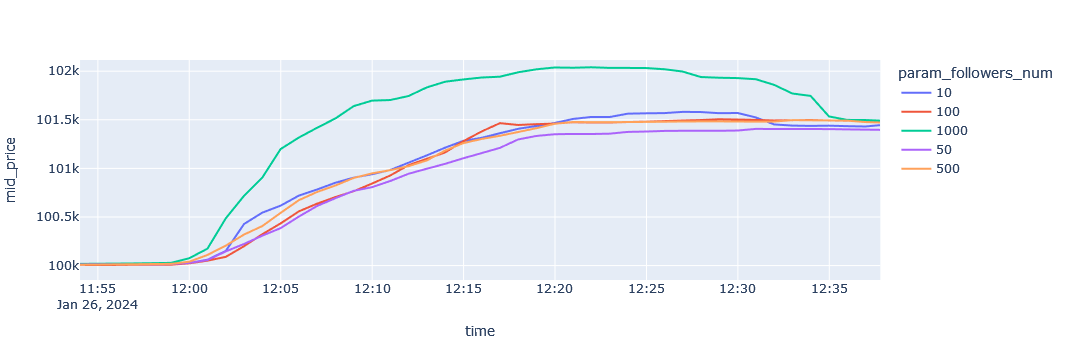
\includegraphics[scale=0.4]{ball.png}
\end{center}
\caption{Średnia cena w replikacji w zależności od liczby agentów typu \textit{FollowerAgent}}\label{fig:ball}
\end{figure}
\end{center}






% 
% wykres ceny w zależności od kapitału dla wybranej replikacji 
% wykres 
\chapter*{Podsumowanie}

Podejście do rozwinięcia modelu agentowego rynku okazało się, nieoczekiwanie, zadaniem wymagającym i interdyscyplinarnym. Powierzchownie nieskomplikowane konstrukcje agentów zawierają elementy zaadaptowane z różnych, często nie wprost powiązanych, dziedzin. 

Po zapoznaniu się z dotychczasowym dorobkiem w dziedzinie modelowania agentowego rynku zdecydowaliśmy się rozwinąć wybrany model referencyjny w kierunku odtworzenia obserwowanego współcześnie zróżnicowanego dostępu do informacji. Zaproponowaliśmy model zbudowany wokół popartego stylizowanymi faktami założenia o bezpośrednim wpływie zdarzeń ekonomicznych na cenę, wprowadzając przy tym dwa nowe podtypy agentów oraz system komunikacji między nimi. Rozwinięty model wykorzystaliśmy do weryfikacji hipotez na temat skutków działań gracza z uprzywilejowaną wiedzą. 

Opisany w pracy model skoncentrowany wokół zdarzenia ekonomicznego oraz towarzyszące mu symulacje i ich analiza w żadnym razie nie wyczerpują tematu nierówności dostępu do informacji na rynkach finansowych. Wręcz przeciwnie - wyniki przeprowadzonych symulacji sygnalizują nowe wątki domagające się rozwinięcia i szerszej analizy. 

 




% \frontmatter defines the pieces of the thesis which will use roman numerals for page numbering



% \chapter{} and/or \chapter*{} will create a chapter in your thesis.  Including the asterisk will cause the chapter to not appear in the table of contents.

% \input will reference a particular .tex file.  Here we are grabbing a file entitled Abstract stored in the 

\newpage
\bibliographystyle{plain}
\bibliography{bibliography}
 % Entries are in the refs.bib file

%% Look!  A mock introduction

The introduction is one of the most important pieces of your thesis.  Here is a place for you to introduce the problem(s) on which you have worked and place them in the larger context of your field.  You should aim to ensure that this section is completely understandable to virtually anyone - and certainly anyone with a sophomore-level grasp of physics.  Presumably this will include references to the literature.

In addition to setting your work into context, a second good idea for your introduction is to give a short outline for what the rest of your thesis will discuss.  This is often done in the closing paragraph(s) of the introduction with sentences like ``In the following chapters \ldots " and ``Chapter 2 discusses \ldots"  Tremendous detail is not required in this outline, but rather just a brief road map for the rest of the document.

\section{A section}

The \texttt{\textbackslash section} tag will create a new section within a chapter.  Sections will be sequenced with digits following a decimal point in the table of contents, i.e. this is section 1.1.

\section{Another section}

This second section is, obviously, 1.2.

\subsection{A subsection}

Subsections are created using the \texttt{\textbackslash subsection} delineate smaller pieces of your document, and will appear after a second decimal point; this is subsection 1 of section 2 of chapter 1, i.e. 1.2.1.

\subsubsection{A subsubsection}

Subsubsections are still smaller sections.  By default, this is the finest subdivision of a chapter in \LaTeX, and they will \emph{not} appear in the table of contents.  

\subsection{A useful command}

\marginpar{This is a margin note.}
One command I often ask my students to use is \texttt{\textbackslash marginpar}, which can be used to create a margin note.  These are super helfpul if there's something to which you need to return later (say, after you've looked up a number), as notes in the margin are really easy to find quickly.  

\section{Some figures}

You will surely want to add figures to your thesis to help explain your ideas.  There are a number of different ways to include such things, but the most typical way would be to generate the figure in another piece of software (\texttt{MATLAB, Mathematica, Adobe Illustrator, \ldots} and simply include it in your \LaTeX ~code.  This will require use of the \emph{figure} environment.\footnote{there are many other possible environments to include figures, such as wrapfigure, but these will require including additional packages \ldots}  See this document's \LaTeX ~code for details . . .

% Here is the figure environment.  The [] after \begin{figure} are an optional argument that tells LaTeX where to try to place the figure.  If you do not include it then it will figure out the `best' place to put things on its own, but on occasion the choices it makes are a bit strange.  Even so, you should probably try to let it make the decisions whenever possible, and only come back to enforce new locations after you have essentially finished your document.  Otherwise you may find that your instructions are no longer appropriate if you add text elsewhere in the document that changes how things are alligned.  Anyhow, [h] instructs LaTeX to put th e figure `here', and adding an exclamation point [h!] means REALLY, PUT IT HERE.  [t] and [b] mean to put the figure at the top or bottom of a page, respectively.
\begin{figure}[h!]

%\centering centers the figure on the page.  This is convention.
\centering

% The \includegraphics command is the default way to include a figure.  The first optional argument in [] brackets defines how large the figure should be on the page.  This can be defined in inches, centimeters, or as a fraction of the \textwidth.  Then, in the curly {} braces you will put the file name for the figure.  Here it has been stored in a subfolder entitled Figures.  You are encouraged to give your figures descriptive file names, as this will help future students to figure out what figure corresponds to which file without having to read your LaTeX code.  
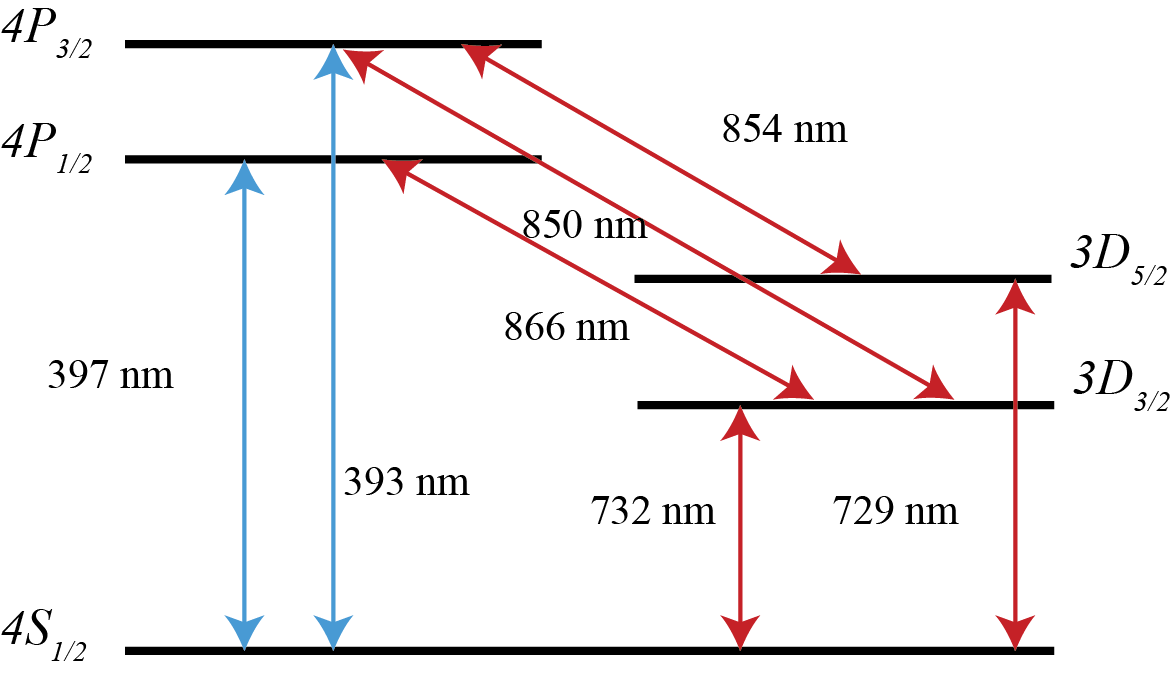
\includegraphics[width=.8\textwidth]{Chapters/Figures/calcium_levels_1-1.PNG}

%\caption will create a figure caption.  Putting an asterisk after it (as in \caption* ) will cause the caption to not be numbered and to not appear in the list of figures.  The [] argument is optional but recommended; this is the short-form caption which will appear in the list of figures.  The {} argument is required, and gives the full caption which will appear in the main text.  The first few words of this caption will be used in the list of figures if no [] form is given.  
\caption[Short-form caption]{Long-form caption that appears in main body of the document}

% the \label gives a reference for this figure so that you can refer to it in the text by its number in a way which will be automatically updated if you change the document.  THIS IS A GOOD IDEA; having automatically updated references for figures, equations, etc, will keep your document in order even as you continue to update it over a period of months.  This reference can be called in the text using the \ref tag.
\label{fig:aFigure}
\end{figure}



Here, back in the main body of the text, we can create a reference to figure \ref{fig:aFigure}.  This is automatic; the actual numbers are not typed into the code, but rather the \texttt{\textbackslash ref} tag has been used.  Always always always use the \texttt{\textbackslash ref} command to reference figures, or invariably at some point you'll move something and all of your references will be incorrect and you'll have to fix them manually.

% Here is the same figure, but now using the wrapfigure environment.  This allows you to wrap your text around the figure itself.  The optional [] argument specifies how many lines of text should be wrapped.  The first {} argument specifies where on the page the figure should live (here the right side is specified).  The second {} argument defines how much real estate on the page will be allocated for the figure block; here it is 45% of the page width.
\begin{wrapfigure}[11]{r}{0.45\textwidth}
\centering
% \vspace creates vertical white space in the document.  Here we are creating 0.1 lines of text worth of negative white space, effectively moving our graphic up in the document by one line.  I find this lines things up better within the text in this case, but you may need to manipulate this to make the alignments look correct.
\vspace{-.1\baselineskip}
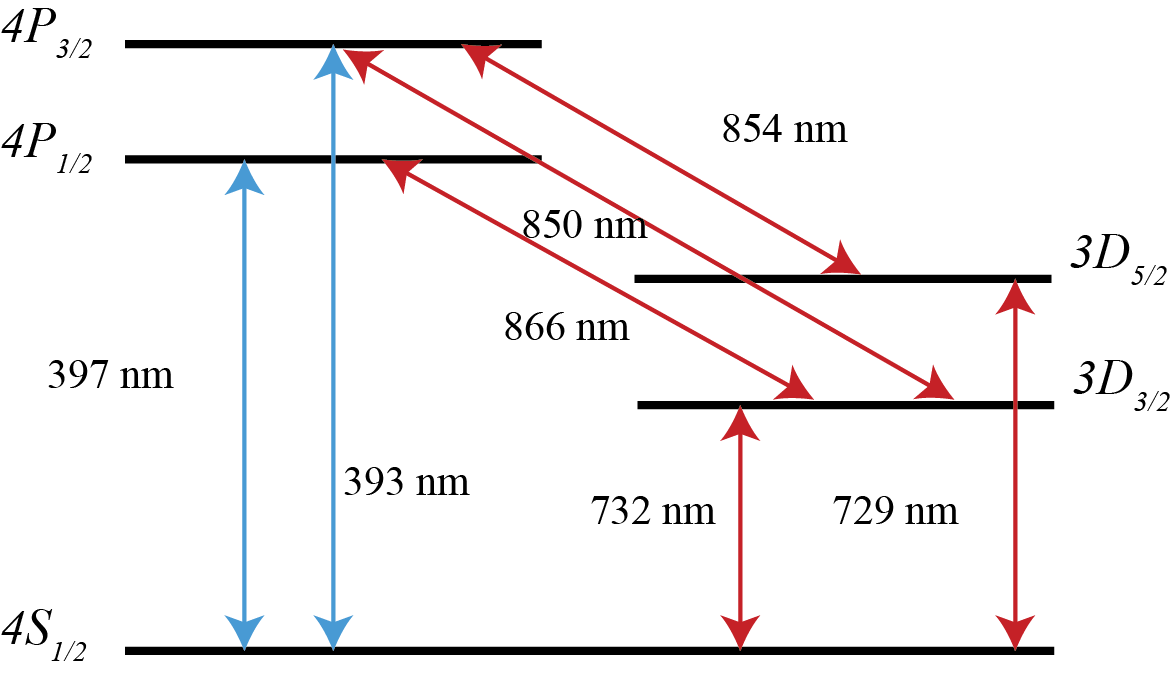
\includegraphics[width=.4\textwidth]{Chapters/Figures/calcium_levels_1-1.PNG}
\caption[Another short-form caption]{A figure included using the wrapfig environment}
\label{fig:anotherFigure}
\end{wrapfigure}
As an alternative to the ordinary figure environment, you might deem it desirable to tuck a figure in more closely amongst the text.  This has a separate environment known as \emph{wrapfig}.  Here we will include the same figure as above a second time, but this time using the \emph{wrapfig} environment.  This will insert the figure into your document with the text wrapping around the perimeter, rather than offsetting it into its own separate chunk of page, as above.    As before, we can use an automated reference to the figure using the \texttt{\textbackslash ref} tag; here we have figure~\ref{fig:anotherFigure}.  Working with the wrapfigure environment sometimes requires a little bit of massaging to ensure that everything lines up properly in your document, but with a small amount of work  you will find that you can get the text to box the figure quite nicely.

Here I have added a table, because tables are also useful. This table has nothing to do with the rest of the material in this thesis template, but you should probably only add relevant tables.
\begin{table}[tbh]
\begin{center}
%\caption[]{\em{Here we show the continuum sensitivity required per band.}}
\begin{tabular}{ccccccc}
\hline \noalign {\smallskip}
Name & SpT & Dist. & Age & 3$\sigma$ M$_{\rm dust}$ & 3$\sigma$ CO(3-2) limit & Disk indicator \\
 & & (pc) & (Myr) & limit (M$_{\oplus}$) &  (mJy km s$^{-1}$)\\
\hline \noalign {\smallskip}
J0226 & L0 & 46.5 & 45 & 0.01 & 24 & Pa$\beta$, IR\\
J0501 & M4.5 & 47.8 & 42 & 0.01 & 23 & H$\alpha$, IR\\
J1546 & M5 & 59.2 & 55 & 0.01 & 14 & HeI, [OI], H$\alpha$, IR\\
J0446 A/B & M6/M6 & 82.6/82.2 & 42 &  0.027 & 18 & H$\alpha$, IR\\
J0949 A/B & M4/M5 & 79.2/78.1 & 45 &  0.024 & 17 & H$\alpha$, IR\\
LDS 5606 A/B & M5/M5 & 84/84 & 30-44 & 0.027 & 19 & H$\alpha$, IR, UV\\
\hline \noalign {\smallskip}
\end{tabular}
\end{center}
\end{table}




%\chapter{A second chapter}
%% Another mock chapter

Here is a second mock chapter.  As far as the \LaTeX ~is concerned, it is in no way different from the introduction excepting that it appears after it in the main .tex file.  As before, it can be populated with sections, subsections, figures, etc. as you see fit.

In fact, you will probably write perhaps three to six chapters for your thesis depending on how your work is most effectively organized.  Most theses will contain an introduction, at least one `body' chapter, and some sort of conclusions/future directions chapter.  Most theses will also include an appendix or two \ldots


% the \appendix tag tells LaTeX where it should start labeling chapters with letters (denoting appendices) rather than numbers (denoting main chapters)
%\appendix 
%%% przepisać
%\chapter{Obrazy}

%\begin{appendices}

%\chapter{Kod}


%\end{appendices}
%% Look!  An Appendix!

Appendices are a good idea for almost any thesis.  Your main thesis body will likely contain perhaps 40-60 pages of text and figures.  You may well write a larger document than this, but chances are that some of the information contained therein, while important, does \emph{not} merit a place in the main body of the document.  This sort of content - peripheral clarifying details, computer code, information of use to future students but not critical to understanding your work \ldots - should be allocated to one or several appendices.  


\section{About the bibliography}
What follows this is the bibliography.  This has its own separate environment and syntax; check out the comments in the .tex files for details.  Worth nothing, though, is that you may find it helpful to use automated bibliography management tools.  BibTeX will automatically generate a bibliography from you if you create a database of references.  Other software - for example JabRef on a pc - can be used to make managing the reference database easy.  Regardless, once you've created a .bib file you can cite it in the body of your thesis using the \texttt{\textbackslash cite} tag.  For example, one might wish to cite a reference by Bermudez \cite{Bermudez}.  If you use BibTeX, you can put the relevant information into a referencedatabase (called bibliography.bib here), and then BibTeX will compile the references into a .bbl file ordered appropriately for your thesis based on when the citations appear in the main document.
%\chapter{Programy}
% wzmianka o repozytorium -> zmienić sobie nick

% \bibliographystyle tells LaTeX how you want to format your bibliography.  There are many standard formats.  apsrev is fairly typical, but feel free to explore other options if the mood strikes.  


% \bibliography calls the actual file that contains your bibliographic information.  This file can be generated by hand or in an automated way using software such as BibTeX.  Either works fine, but it is worth learning to use BibTex in the long term.  Take a look at the .bib file included here if you want to get some idea of the formatting required to create a bibliogrphy file of your own.


\end{document}